%---------------------------------------------------------------------------%
%-                                                                         -%
%-                           LaTeX Template                                -%
%-                                                                         -%
%---------------------------------------------------------------------------%
%- Copyright (C) Huangrui Mo <huangrui.mo@gmail.com> 
%- This is free software: you can redistribute it and/or modify it
%- under the terms of the GNU General Public License as published by
%- the Free Software Foundation, either version 3 of the License, or
%- (at your option) any later version.
%---------------------------------------------------------------------------%
%->> Document class declaration
%---------------------------------------------------------------------------%
\documentclass{Style/ucasproposal}%
%- Multiple optional arguments:
%- [<oneside|twoside|print>]% oneside eprint, twoside eprint, or paper print
%- [fontset=<adobe|none|...>]% specify font set instead of automatic detection
%- [scheme=plain]% thesis writing of international students
%- [draftversion]% show draft version information
%- [standard options for ctex article class: draft|paper size|font size|...]%
%---------------------------------------------------------------------------%
%->> Document settings
%---------------------------------------------------------------------------%
\usepackage[authoryear,xhf,tikz,table]{Style/artratex}% document settings
%- usage: \usepackage[option1,option2,...,optionN]{artratex}
%- Multiple optional arguments:
%- [bibtex|biber]% set bibliography processor and package
%- [<numbers|super|authoryear|alpha>]% set citation and reference style
%- <numbers>: textual: Jones [1]; parenthetical: [1]
%- <super>: textual: Jones superscript [1]; parenthetical: superscript [1]
%- <authoryear>: textual: Jones (1995); parenthetical: (Jones, 1995)
%- <alpha>: textual: not available; parenthetical: [Jon95]
%- [geometry]% reconfigure page layout via geometry package
%- [lscape]% provide landscape layout environment
%- [xhf]% disable header and footer via fancyhdr package
%- [color]% provide color support via xcolor package
%- [background]% enable page background
%- [tikz]% provide complex diagrams via tikz package
%- [table]% provide complex tables via ctable package
%- [list]% provide enhanced list environments for algorithm and coding
%- [math]% enable some extra math packages
%- [xlink]% disable link colors
\usepackage{Style/artracom}% user defined commands
%---------------------------------------------------------------------------%
%->> Project-wide notation
%---------------------------------------------------------------------------%
\newcommand{\earlyinside}{\textsc{Early-Inside}}
\newcommand{\gatedinside}{\textsc{Admission-Gated Inside}}
\newcommand{\serialsplit}{\textsc{Serial-Split}}
\newcommand{\pdlsplit}{\textsc{Split+PDL}}
\newcommand{\microsecond}{\ensuremath{\,\mu\mathrm{s}}}
\newcommand{\TE}{\ensuremath{T_{\mathrm{E}}}}
\newcommand{\TG}{\ensuremath{T_{\mathrm{G}}}}
\newcommand{\TS}{\ensuremath{T_{\mathrm{S}}}}
\usepackage{enumitem}
\usepackage{makecell}
\usepackage{float}
\newcommand{\us}{\,\textmu s}
\newcommand{\rcite}[2]{#2}
\newcommand{\refitem}[1]{\item}
\newcommand{\cQiang}{\rcite{qiang2026}{Qiang 等 (2026b)}}
\newcommand{\cChat}{\rcite{chatterjee2026}{Chatterjee 等 (2026a)}}
\newcommand{\cHazy}{\rcite{spector2025}{Spector 等 (2025b)}；\rcite{hazy2025b}{Hazy Research (2025)}}
\newcommand{\cMPK}{\rcite{cheng2026}{Cheng 等 (2026)}}
\newcommand{\cVllm}{\rcite{kwon2023}{Kwon 等 (2023)}}
\newcommand{\cFA}{\rcite{dao2024}{Dao (2024)}}
\newcommand{\cGraph}{\rcite{nvidia2026a}{NVIDIA (2026a)}}
\newcommand{\cPDL}{\rcite{nvidia2026b}{NVIDIA (2026b)}}
\newcommand{\cDacos}{\rcite{hao2026}{Hao 等 (2026)}}
%---------------------------------------------------------------------------%
%->> Document inclusion
%---------------------------------------------------------------------------%
%\includeonly{Tex/Chap_1,...,Tex/Chap_N}% selected files compilation
%---------------------------------------------------------------------------%
%->> Document content
%---------------------------------------------------------------------------%
%-
%-> Titlepage information
%-
%---------------------------------------------------------------------------%
%->> Titlepage information
%---------------------------------------------------------------------------%
%-
%-> 中文封面信息
%-
\schoollogo{scale=0.112}{ucas_logo}% 校徽
\title[面向低时延大语言模型推理的计算图自适应执行机制研究]{面向低时延大语言模型推理的计算图\\自适应执行机制与跨边界重叠研究}% 题目
\author{郝朝阳}% 作者姓名
\authorid{2024E8013282103}% 学号
\advisor{赵家程}% 指导老师
\advisortitle{副研究员}% 指导老师职务
\degree{硕士}% 学位：硕士、博士
\degreetype{工学}% 学位类别：理学、工学、工程、医学等
\major{计算机科学与技术}% 二级学科专业名称
\field{AI 编译器与 GPU 高性能计算}% 研究方向
\institute{处理器芯片全国重点实验室}% 院所
\chinesedate{2026~年~11~月}% 日期
%---------------------------------------------------------------------------%
%
\begin{document}
%-
%-> Frontmatter: title page, abstract, content list, symbol list, preface
%-
\pagenumbering{roman}% page numbers with roman style
%---------------------------------------------------------------------------%
%-> Frontmatter
%---------------------------------------------------------------------------%
%-
%-> 生成封面
%-
\maketitle% 生成中文封面
%-
%-> 目录
%-
\tableofcontents% 生成目录
%---------------------------------------------------------------------------%
% title page, abstract
%-
%-> Mainmatter
%-
\clearpage
\pagenumbering{arabic}% restart page numbers with arabic style
%---------------------------------------------------------------------------%
%->> Main content
%---------------------------------------------------------------------------%

\section{课题目标与计划执行情况总结}
\subsection{课题目标}
\label{sec:purpose}

本课题研究低时延大语言模型推理中相邻算子之间的执行方式。计算图上的每一条边都面临同一个选择：生产者与消费者留在同一 grid 内，还是分属两个 grid、在二者之间形成物理边界；若形成物理边界，后继是否借助 Programmatic Dependent Launch（PDL）提前启动，与前驱重叠。开题报告把这一选择表述为全图执行计划的优化
\begin{equation}
\Pi^{\star}(G,x)=\arg\min_{\Pi\in\mathcal{F}(G,x)} T(G,x;\Pi), \label{eq:obj}
\end{equation}
其中 $G=(O,E)$ 为计算图，$x$ 为输入规模与运行配置，$\Pi$ 为各边处理方案 $\pi(e)=\langle m_e,\theta_e\rangle$ 的集合，$\mathcal{F}(G,x)$ 为满足数据依赖、内存可见性与硬件资源约束的合法计划集合。围绕式~(\ref{eq:obj})，开题报告确定了四项研究内容：计算图依赖关系建模、依赖感知的 PDL 跨边界重叠、全图边处理方案搜索，以及框架实现与端到端验证。

\subsection{计划执行情况}

按开题计划，至 2026 年 11 月应完成前两项研究内容并启动第三项。实际执行情况如表~\ref{tab:plan} 所示：前两项的主体工作已按计划完成；第三项完成了 decoder layer 链上的规划器及其与固定方案的实测比较；第四项提前启动，已建立统一算子后端，并贯通 prefill 与单步 decode 的正确性通路。

\begin{table}[htbp]\centering
\caption{研究计划执行情况}\label{tab:plan}
\small
\begin{tabularx}{\textwidth}{@{}p{3.3cm}p{2.1cm}X@{}}
\toprule
研究内容 & 计划时间 & 完成情况\\
\midrule
计算图依赖关系建模 & 2026.07–08 & 基本完成。建立阶段级依赖抽象、逐边合法候选与 grid 资源包络模型；task/tile 级就绪粒度在 Hazy Megakernels 原型上完成验证；面向任意计算图的 lowering 尚未形成独立模块。\\
依赖感知的 PDL 跨边界重叠 & 2026.09–10 & 基本完成。实现触发、同步与权重预取的参数化 PDL 交接，完成逐边 PDL 选择与边级实测，给出后继提前进入的条件、落位的派发模型与不依赖逐边实测的选择判据；触发时机与预取量目前取固定值。\\
全图边处理方案搜索 & 2026.11–12 & 进行中。完成 32 种分组方式的枚举式规划器与实测校验；建立矩阵阶段、attention 与多阶段分组的时延模型并接入规划器，以约四成的测量量得到时延相当的方案；在 15 个负载上完成各项决策对输入规模依赖的分类；层间异构方案、候选计划表与在线选择尚未完成。\\
框架实现与端到端验证 & 2027.01–04 & 提前启动。完成统一算子后端与 prefill、单步 decode 的数值校验；连续 token 生成与 TPOT 分位数尚未完成。\\
\bottomrule
\end{tabularx}
\end{table}

相对开题报告，研究过程中作了两点调整。其一，边处理参数 $\theta_e$ 由同步与 PDL 参数扩展到 grid 级资源配置。实验表明，一条边是否应成为物理边界，主要取决于两侧算子共享同一 launch 资源包络所付出的代价（第~\ref{sec:hw}~节），因此线程块数、分块形状与分阶段驻留配置须与边界选择一并决定。其二，评测目标由 decode 单步扩展到 prefill 与 decode 两个阶段。两个阶段中各算子的时延占比与资源需求不同，同一条边的最优处理方式随之变化，仅以稳态 decode 评测不足以反映首 token 时延。

\subsection{已取得的阶段性成果}

\begin{enumerate}[leftmargin=2.6em,itemsep=2pt]
\item 建立了阶段级的边处理抽象与 grid 资源包络模型，将分块形状、线程块数与分阶段驻留配置纳入边处理参数，并以共驻代价给出是否切分的判据。
\item 完成了 H100 上边界交接代价、访存带宽、阶段并行度需求、线程块放置与主循环构成的定量分析，查明小分块的主循环受访存一侧限制。
\item 实现了统一算子后端、同 grid 内的分阶段驻留配置与参数化的 PDL 交接，全部方案通过数值校验。
\item 实现了逐边规划器。相对充分调优的单一 grid，规划方案在 decode 上最高降低 13.0\% 的单步时延，在 prefill 上最高降低 19.2\% 的首 token 时延；在资源需求相近的负载上规划器保留单一 grid。
\item 建立了矩阵阶段、attention 与多阶段分组的时延模型：矩阵阶段在 40 个留出行数上的中位误差为 3.4\%–3.9\%，分组模型在 2177 组实测配置上为 4.9\%。
\item 给出了 PDL 下以 carve-out 档位与资源余量表述的准入条件、档位沿发射链保持的规律与后继落位的派发模型，并据此划分三类边界；后继以矩阵阶段开头时，判为均衡的 113 类实测边界中 94\% 因 PDL 加速。加入 L1 判据后，按判据选择 PDL 与逐边搜索所得的时延降幅中位数相近。
\item 把代价模型与 PDL 判据接入规划器，以穷举式规划 43\% 的测量量得到时延相差不超过 1.0\% 的方案。
\item 在 15 个负载、1649 个端到端方案上测量了各项决策对输入规模的依赖，据此把决策分为固定型、切换型与参数型：decode 上边的切分可以离线固定，prefill 上只需两个机制候选（最大损失 0.6\%），各组的资源配置须按约 22 个行数区间确定；并给出离线准备、在线查表的系统结构。
\end{enumerate}


\subsection{存在的问题}\label{sec:issues}

\begin{enumerate}[leftmargin=2.6em,itemsep=2pt]
\item \textbf{收益集中于部分负载。}batch 为 1 的短上下文 decode 与最短的 prefill 中，各阶段的资源需求相近，单一 grid 仍是最优方案，规划方案的收益不超过 0.3\%。这些负载恰是低时延场景的典型工作点；其上可能的改进来自同 grid 内的细粒度事件范式，而该范式尚未并入统一后端。
\item \textbf{算子实现仍有差距。}batch 为 1 的 decode 比 Hazy Megakernels 慢 26\%；行数不小于 256 的 prefill 中，后端的 GEMM 落后于 cuBLAS，规划方案比逐算子 CUDA Graph 慢 28\%–73\%。边处理方式的结论建立在同一后端内部的比较之上，但端到端的绝对时延受此限制。
\item \textbf{依赖抽象的粒度与通用性不足。}当前抽象停留在阶段级，分组方式各层相同，候选空间为 32 种；task/tile 级的就绪事件只在 Hazy Megakernels 原型上验证过，面向任意计算图的 lowering 尚未形成独立模块。
\item \textbf{模型的精度只够排序。}分组模型在含 attention 的 prefill 分组上的中位误差为 8.0\%–15.3\%，对分阶段驻留配置的估计偏乐观；模型引导的规划器因此仍需实测排在前列的配置与全部单阶段分组，测量量为穷举式的 43\%，个别负载上所得方案比穷举式方案慢 1.0\%。含 embedding 与词表投影的分组尚无模型，这些分组仍测全部配置。
\item \textbf{集中放置的减速幅度尚无解析式。}派发模型可以预测后继的落位，探针作为 PDL 后继运行时也能复现真实方案中 U 的减速（5.3–7.2 对 7.6\us），但减速随各 SM 上线程块数的分布而变，目前只有“读取带宽在 SM 之间的分配不与线程块数成正比”这一定性规律，没有由分布直接给出时延的公式；真实方案中部分层的后继均匀地落在 64 个 SM 上（每个 SM 2 个），执行时间仍增加约三成，这一部分尚未解释。规划时这不影响取舍，因为可能被集中放置的边界不启用 PDL。可共驻的边界上，运行时常使少数 SM 多驻留一个线程块，模型对这类边界的命中率为 134/172。
\item \textbf{L1 敏感度按负载取得。}attention 对 L1 容量的敏感度随序列长度变化，目前由每个负载上一次强制档位的运行测得，尚未写成序列长度的函数；carve-out 作为分组的配置项也尚未进入搜索。attention 分组每个 SM 只能驻留 4 个线程块的原因仍未查明。
\item \textbf{硬件性能计数器不可用。}实验平台的计数器仅对管理员开放，主循环内逐指令的停顿归因无法取得，图~\ref{fig:ablate} 的消融只能给出部件一级的结论。
\item \textbf{评测负载的行数未覆盖分块边界。}第~\ref{sec:exp}~节的 15 个负载的行数均为分块行数的整倍数，而行数刚越过整倍数时矩阵阶段的时延可升高 47\%（第~\ref{sec:cm}~节），真实请求的行数并不受此约束。
\item \textbf{端到端验证不完整。}评测限于 prefill 与单步 decode，尚未接入连续 token 生成，也未报告 TPOT 与 P50/P90/P99；模型与硬件各只有一种。
\item \textbf{决策分类的覆盖范围有限。}三类决策的划分建立在 15 个负载之上，矩阵阶段的行数区间取自合成驱动上的单阶段分组；二者尚未扩展到 batch 与序列长度的网格和多阶段分组。候选计划表与在线阶段尚未实现，查表与切换计划的开销没有实测数据。
\end{enumerate}



\section{现有研究进展}
围绕第 1 章确立的总体目标（式~(\ref{eq:obj})）与四个核心问题，本章依次汇报中期阶段已完成的研究进展：第~\ref{sec:dep}~节从通用计算图 $G=(O,E)$ 出发，说明如何将原始算子图化简为阶段依赖图，并结合单次 kernel 启动的硬件资源约束统一表示执行计划；第~\ref{sec:pos}~节系统对比 Persistent Kernel 与独立 Kernel 两类执行方式的优缺点与适用条件，归纳边界选择的关键硬件因素；第~\ref{sec:mech}~节介绍统一 CUDA 算子实现、基于前期工作 DACOS 的 PDL 跨边界重叠及静态启用规则；第~\ref{sec:search_sys}~节阐述基于线程块波次的耗时解析模型、引导式离线规划方法与动态 shape 自适应架构；第~\ref{sec:exp}~节在真实大模型和语料上汇报端到端与模块级实验评估结果。

\subsection{算子间依赖分析与片上资源约束建模}\label{sec:dep}\label{sec:abs}

本节回答问题一：面对输入的推理计算图 $G=(O,E)$，如何在不过度绑定特定模型的前提下完成算子间数据依赖分析，并将跨 kernel 执行决策与 GPU 片上资源约束纳入同一表示？

\subsubsection{从通用算子计算图到阶段级依赖抽象}\label{sec:form}

在第 1 章的问题建模中，系统的输入是任意推理计算图 $G=(O,E)$，其中每个节点 $o\in O$ 是一个原始算子（如矩阵乘、注意力、归一化、激活、位置编码、残差相加等）。但在实际优化时，并不需要对原始计算图里的每一条边都做“是否切分为独立 kernel”的决策。从 GPU 执行特征看，深度学习推理计算图中的算子天然分为两类：
\begin{itemize}[leftmargin=2.0em,itemsep=2pt]
\item \textbf{计算或归约主导算子}（如线性投影 GEMM、Attention 等）：计算量或访存量大，通常需要专门的矩阵分块、共享内存双缓冲和较高的寄存器预算，且不同算子偏好的线程块并行度差异显著；
\item \textbf{访存主导的轻量逐元素/尾处理算子}（如 RMSNorm、RoPE、SwiGLU/SiLU 激活、残差相加、KV 缓存写入等）：计算量极小，将它们单独拆成独立 kernel 既不能缓解寄存器或共享内存压力，反而必然带来额外的全局内存读写和 kernel 启动开销。
\end{itemize}

基于这一共性规律，本课题对任意输入计算图 $G=(O,E)$ 首先执行一道\textbf{与具体模型无关的轻量算子吸收（prologue/epilogue 预融合）}：将轻量逐元素与尾处理算子直接并入相邻主导算子的输入准备或输出收尾阶段，从而把原始算子图 $G=(O,E)$ 化简为由主导计算阶段构成的\textbf{阶段依赖图} $G_S=(V_S,E_S)$。真正存在“融合为同一 kernel”与“切分为独立 kernel”硬件权衡的，正是阶段图中的相邻阶段边 $e=(u,v)\in E_S$。需要强调的是，这套从 $G=(O,E)$ 到 $G_S=(V_S,E_S)$ 的化简与建模方法并不局限于某一种特定网络：若换成 Qwen、Gemma、Mistral 等不同归一化或激活形式的模型，或是包含路由与专家分组 GEMM 的 MoE 模型、多头潜在注意力（MLA）及混合架构，化简后仅是阶段图 $G_S$ 的节点类型与连接关系随之变化，后续的依赖分析、资源约束建模、PDL 重叠和方案搜索流程均直接作用在 $G_S$ 上，无需针对单一模型硬编码固定阶段数。

在中期真机实验验证中，课题以主流轻量化模型 Llama-3.2-1B（16 个解码层，隐藏维度 2048，中间层维度 8192，32 个查询头与 8 个键值头）作为具体实例。将上述通用化简规则作用于 Llama 解码层后，每层自然归结为五个顺序主导阶段：Q 阶段（输入 RMSNorm、QKV 线性投影、RoPE 位置编码与 KV cache 写入）、A 阶段（attention 计算）、O 阶段（输出投影、残差相加与后继 RMSNorm）、U 阶段（gate/up 投影并在寄存器内融合 SwiGLU 激活）以及 D 阶段（down 投影、残差相加与下一层输入 RMSNorm）；全模型首层前接词嵌入（embedding），末层后接词表投影与贪心采样（argmax）。层内与跨层相邻阶段由此构成五类核心算子边：Q$\to$A、A$\to$O、O$\to$U、U$\to$D 以及跨层边 D$\to$Q。

对应第 1 章中的任务级依赖分析，对阶段图中的任意依赖边 $e=(K_i,K_j)\in E_S$，系统同时分析两方面信息：一是\textbf{数据就绪粒度}，即后继 $K_j$ 的某个任务是仅需前驱局部输出即可开始（局部就绪），还是必须等待前驱全部输出完成（全量就绪）；二是沿用前期工作 DACOS~\pDacos 对跨 kernel 输入的划分，将后继 $K_j$ 的输入拆分为前驱实时产出的\textbf{依赖张量}与启动时刻即已就绪的\textbf{独立张量}（如只读权重、张量描述符与索引元数据），进而提取出可在首次读取依赖数据前合法提前执行的\textbf{独立前缀}。表~\ref{tab:edges} 给出了 Llama-3.2-1B 实例下五类阶段边的依赖形态与独立前缀。

\begin{table}[!htb]\centering
\caption{Llama-3.2-1B 解码层实例中五类相邻阶段边的依赖就绪形态与消费者独立前缀}\label{tab:edges}
\small
\begin{tabularx}{\textwidth}{@{}p{1.4cm}>{\raggedright\arraybackslash}p{6.5cm}>{\raggedright\arraybackslash}X@{}}
\toprule
算子边 & 数据依赖就绪形态 & 消费者可提前执行的独立前缀\\
\midrule
Q$\to$A & 局部就绪：各 KV 头分组的 attention 仅依赖对应头的 Q、K、V 输出 & 历史缓存 KV 块的异步读取（decode 阶段）\\
A$\to$O & 全量就绪：输出投影的每个分块均依赖全部查询头的完整聚合结果 & 输出投影权重（8\,MiB）的片外预取\\
O$\to$U & 全量就绪：每个输出分块依赖前驱在对应 token 行上的完整归一化输出 & Gate/up 投影权重（64\,MiB）的片外预取\\
U$\to$D & 全量就绪：down 投影沿中间维度归约，依赖完整的激活张量 & Down 投影权重（32\,MiB）的片外预取\\
D$\to$Q & 全量就绪：下一层 QKV 投影依赖完整的层间归一化激活 & 下一层 QKV 权重（12\,MiB）的片外预取\\
\bottomrule
\end{tabularx}
\end{table}

对应第 1 章定义的边级候选空间 $\mathcal{M}(e)$，阶段图中的每条边 $e\in E_S$ 可选用三类物理执行方式（图~\ref{fig:scheme}）：
\begin{enumerate}[leftmargin=2.4em,itemsep=2pt]
\item \textbf{同 grid 融合}：将前后阶段编译进同一个 persistent grid，靠设备端全局屏障保证全局内存可见；
\item \textbf{跨 grid completion（串行切分）}：在该边切分为两个独立 kernel，等待前驱全部线程块退出后再启动后继；
\item \textbf{跨 grid PDL（切分并重叠）}：保留物理切分边界，由前驱在尾部发出 programmatic completion 信号提前启动后继，让后继先执行独立前缀再等待前驱数据就绪。
\end{enumerate}

针对开题提到的“同 grid 细粒度事件”形态，课题前期也在 Hazy Megakernels 原型\pHazy 上做了对比测试：在 1024 上下文单请求 decode 中，为 QKV 保留按头局部就绪、为 gate/up 采用全量就绪的混合配置可比逐边贪心缩短 11.4--12.7\us（1136.3\us）；但同一原型上的对照同时表明，若各阶段线程块和资源配置保持不变、单纯把单 kernel 拆成多 kernel，时延反而升至 1185.6\us，只有同步重新配置切分后各组的资源参数，PDL 才能把粗粒度切分从串行的 1419.1\us 压低至 1291.9\us。这一现象说明：\textbf{是否切分某条算子边不能脱离硬件资源配置孤立决定，必须与 GPU 单次 kernel 启动的片上资源约束联合建模。}

\begin{figure}[!htb]\centering
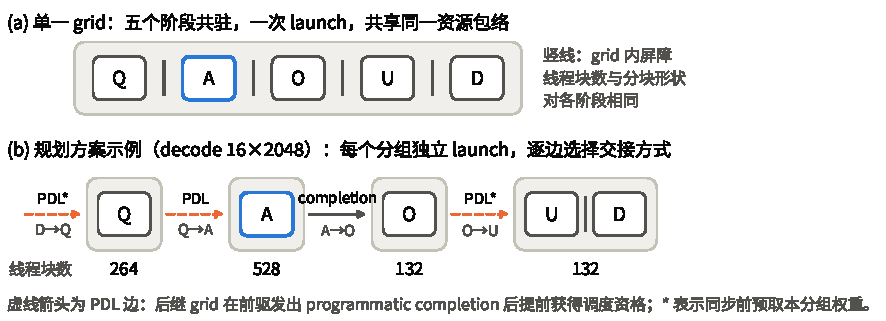
\includegraphics[width=\textwidth]{Img/midterm/scheme}
\caption{阶段依赖图及其边级执行映射示例。(a) 单一 persistent grid 方案下，五个阶段通过核内屏障顺序衔接，共享同一套寄存器与共享内存上限；(b) 针对 decode 16$\times$2048 选出的混合执行计划：attention 独立成组并扩展至 528 个线程块，U 与 D 保持同 grid 融合，四条物理边界中有三条启用跨边界 PDL 重叠。}\label{fig:scheme}
\end{figure}

\subsubsection{单次 Kernel 启动的资源约束与全图执行计划表示}\label{sec:env}

从 GPU 硬件执行模型看，每个线程占用的寄存器数量和每个线程块占用的共享内存大小，都是以\textbf{单次物理 kernel 启动（launch）}为粒度在编译和启动时静态锁定的。当多个连续阶段被融合进同一个物理 grid $g$ 时，整个 kernel 必须按组内需求最苛刻的阶段来分配片上资源：
\begin{equation}
r(g)\ge\max_{s\in g} r_s,\qquad m(g)=\max_{s\in g} m_s. \label{eq:env}
\end{equation}
设单个流多处理器（SM）的寄存器文件容量为 $R_{\mathrm{SM}}$、共享内存容量为 $M_{\mathrm{SM}}$、最大常驻线程数为 $T_{\mathrm{SM}}$（NVIDIA H100 上分别为 65\,536、228\,KiB 与 2048），每线程块包含 $\tau=128$ 个线程时，单个 SM 最多能同时驻留的线程块数 $n(g)$（即 occupancy 上限）由三者中的最小值决定：
\begin{equation}
n(g)\le\min\Bigl(\Bigl\lfloor\frac{R_{\mathrm{SM}}}{\tau\, r(g)}\Bigr\rfloor,\ \Bigl\lfloor\frac{M_{\mathrm{SM}}}{m(g)}\Bigr\rfloor,\ \Bigl\lfloor\frac{T_{\mathrm{SM}}}{\tau}\Bigr\rfloor\Bigr), \label{eq:occ}
\end{equation}
使用协作启动（cooperative launch）时，全卡同时运行的总线程块数不得超过 $n(g)$ 与设备 SM 总数（132）之积。

据此，第 1 章式~(\ref{eq:obj}) 中的全图执行计划 $\Pi$ 在阶段图 $G_S=(V_S,E_S)$ 上可以明确写为三元组 $\Pi=\langle C,\allowbreak \{\theta_g\},\allowbreak \{\varphi_e\}\rangle$：其中 $C\subseteq E_S$ 为切分为物理 kernel 边界的边集合（切分后将阶段图划为若干连续分组 $g$；在 Llama 每层五类边同构取值下共有 $2^5=32$ 种切分方案，$C=\varnothing$ 即退化为全图单一 persistent kernel）；$\theta_g$ 为分组 $g$ 的执行配置，包含矩阵分块形状、启动线程块数及核内各阶段活跃块配置；$\varphi_e\in\{\text{completion},\allowbreak \text{PDL},\allowbreak \text{PDL}^*\}$ 为物理边界 $e\in C$ 的跨核衔接方式（$\text{PDL}^*$ 表示等待前驱数据前附带静态权重预加载）。

\subsection{Persistent Kernel 与独立 Kernel 的优缺点剖析及边界选择因素}\label{sec:pos}

在统一建模的基础上，本节回答问题二：全图融合（Persistent Kernel）与独立切分（Split Kernel）各自的优势和瓶颈究竟在哪里？为什么不同算子边界、不同输入规模需要选择不同的执行方式？

\subsubsection{Persistent Kernel 的优势与资源耦合瓶颈}\label{sec:hw}

Persistent Kernel 将多个连续计算阶段甚至整网融合进同一个物理 grid，整次前向只需启动一次 kernel，常驻 SM 的线程块之间通过设备端同步屏障衔接。它的核心优势非常直接：\textbf{完全消除了主机侧反复提交 kernel 的开销，也避免了相邻 kernel 之间“等待前驱全部退出再重新启动后继”的空闲间隙}。因此，当各阶段所需的线程块数与片上资源需求比较接近时，单一 persistent kernel 确实最快。如表~\ref{tab:cores} 所示，在单请求短上下文 decode（$1\times 512$）和采用轻量逐 warp attention 的极短 prefill（$1\times 16$）上，五阶段融合执行的单层耗时比五阶段各自独立最优之和分别还快 1.3\us 和 1.8\us。

然而，一旦进入长上下文、中大批量或重度算子区间，单一 persistent kernel 就会明显变慢。慢的原因是什么？我们首先通过图~\ref{fig:hw} 的受控微基准排除了“同步原语开销”的猜测：放进 CUDA Graph 封装后~\pGraph，两个空阶段之间无论是用核内全局屏障、跨 grid 串行 completion 还是跨 grid PDL，132 个线程块下的单次同步耗时都在 1.16\us 左右，扩展到 528 块也仅在 1.40--1.88\us 之间（图~\ref{fig:hw}(a)）；同时，流式读取 64\,MiB 线性权重在 264 个线程块（每 SM 2 块，6 级异步流水）处就已吃满 H100 的 HBM 带宽（2.4--3.0\,TB/s，图~\ref{fig:hw}(b)）。这说明，单一 persistent kernel 变慢的真正根源并非同步本身，而是式~(\ref{eq:env})--(\ref{eq:occ}) 揭示的\textbf{不同阶段共享同一片上资源上限造成的冲突}。

\begin{figure}[!htb]\centering
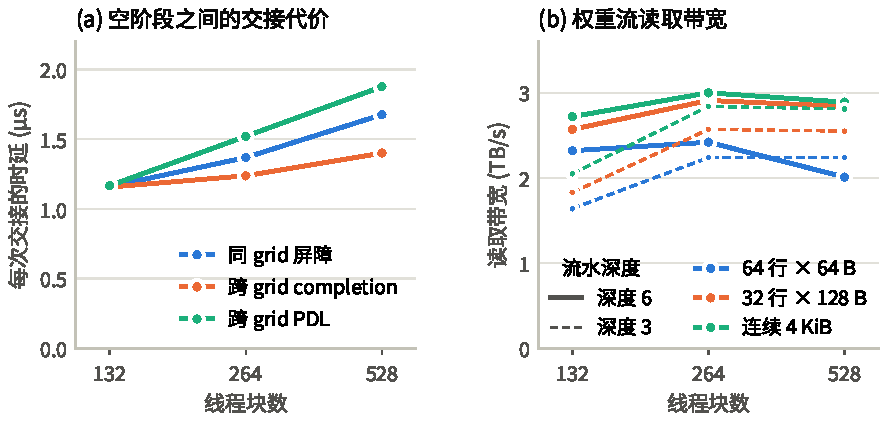
\includegraphics[width=\textwidth]{Img/midterm/hw_micro}
\caption{跨阶段同步开销与流式权重读取带宽微基准。(a) 相邻空阶段间三种衔接方式随线程块数的单次耗时；(b) 流式读取 64\,MiB gate/up 权重的有效带宽随线程块数与访存连续性的变化，在 264 个线程块处即达到平台带宽上限。}\label{fig:hw}
\end{figure}

具体到线性矩阵阶段（Q、O、U、D）与 attention 阶段（A），二者在理想线程块数与片上资源占用上存在两重明显矛盾（图~\ref{fig:stage} 与表~\ref{tab:foot}）：
\begin{enumerate}[leftmargin=2.4em,itemsep=2pt]
\item \textbf{最优线程块并行度相反。}四个矩阵阶段独立运行时普遍在 132 或 264 个线程块处最快，继续增加线程块反而加剧缓存竞争与归约成本；而高负载 decode attention 随线程块数增加显著提速（例如 $16\times 2048$ 下 528 块比 132 块快 2.5 倍）。
\item \textbf{寄存器与共享内存互相拖累。}在 decode 中，矩阵阶段每块需要 72\,KiB 共享内存，将五阶段融合 kernel 的单 SM 并发上限压在 3 块（全卡 396 块），使原本能跑 4 块/SM（528 块）的 attention 损失了四分之一并发度；在 prefill 中，基于 Tensor Core 的 FlashAttention-2~\pFA 每线程用满 255 个寄存器，一旦与矩阵阶段融合，全图所有阶段的并发度都会被拉低到每 SM 2 块（264 块）。
\end{enumerate}

\begin{figure}[!htb]\centering
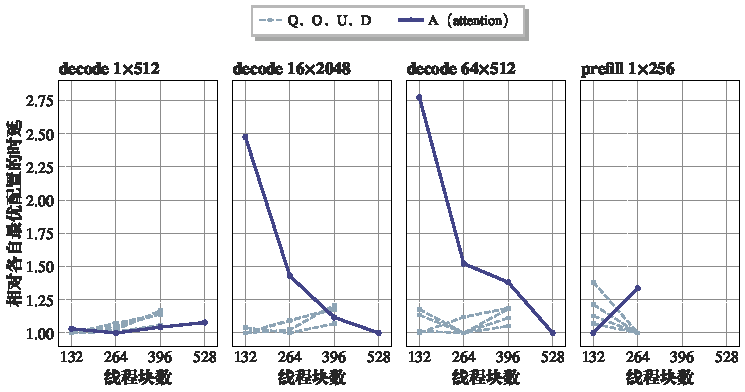
\includegraphics[width=\textwidth]{Img/midterm/stage_ctas}
\caption{矩阵阶段与 attention 阶段独立运行时的最优线程块并行度差异。纵轴为归一化至各阶段最优配置的相对时延；矩阵阶段偏好 132--264 个线程块，而高负载 decode attention 随线程块数扩展至 528 持续提速。}\label{fig:stage}
\end{figure}

\begin{table}[!htb]\centering
\caption{各阶段独立编译与五阶段融合时的静态片上资源需求对比。寄存器按每线程计，共享内存（KiB）按每线程块计，“块/SM”为协作启动单 SM 最大并发线程块数}\label{tab:foot}
\footnotesize\setlength{\tabcolsep}{4.5pt}
\begin{tabular}{@{}lccc@{\hspace{1.4em}}ccc@{\hspace{1.4em}}ccc@{}}
\toprule
 & \multicolumn{3}{c}{Decode（128$\times$16）} & \multicolumn{3}{c}{Prefill，FA2（64$\times$64）} & \multicolumn{3}{c}{Prefill，逐 warp（64$\times$64）}\\
\cmidrule(r{1.4em}){2-4}\cmidrule(r{1.4em}){5-7}\cmidrule{8-10}
阶段或分组 & 寄存器 & KiB & 块/SM & 寄存器 & KiB & 块/SM & 寄存器 & KiB & 块/SM\\
\midrule
Q 阶段 & 124 & 72 & 3 & 158 & 64 & 3 & 158 & 64 & 3 \\
A 阶段 & 124 & 16 & 4 & 255 & 48 & 2 & 48 & 0 & 4 \\
O 阶段 & 122 & 72 & 3 & 150 & 64 & 3 & 150 & 64 & 3 \\
U 阶段 & 112 & 72 & 3 & 144 & 64 & 3 & 144 & 64 & 3 \\
D 阶段 & 122 & 72 & 3 & 150 & 64 & 3 & 150 & 64 & 3 \\
五阶段融合 & 162 & 72 & 3 & 255 & 64 & 2 & 168 & 64 & 3 \\
\bottomrule
\end{tabular}
\end{table}

为了定量衡量这种资源冲突带来的损失，定义单层\textbf{共驻代价}为“五阶段融合在最优单一 grid 中的单层耗时”减去“五阶段各自独立成组并分别取最优配置时的耗时之和（已包含独立启动开销）”。表~\ref{tab:cores} 清楚显示：在重载 decode（$+10.2$ 至 $+21.4$\us/层）、含 FlashAttention-2 的 prefill（$+13.7$ 至 $+40.6$\us/层）以及不同矩阵阶段偏好不同分块的中等规模 prefill（$16\times 16$ 下达 $+25.2$\us/层）上，强行融合付出的资源受限代价远高于微秒级的跨 kernel 启动开销。

\begin{table}[!htb]\centering
\caption{单层耗时分解与融合共驻代价实测对比（\textmu s）。共驻代价为正表示多阶段共享片上资源上限带来的损失超过独立切分的启动开销}\label{tab:cores}
\footnotesize\setlength{\tabcolsep}{4.5pt}
\begin{tabular}{@{}lrrrrrrrr@{}}
\toprule
典型负载 & Q & A & O & U & D & 独立最优之和 & 五阶段融合 & 共驻代价\\
\midrule
decode 1$\times$512 & 9.9 & 8.3 & 11.0 & 26.2 & 19.6 & 75.0 & 73.7 & $-1.3$ \\
decode 4$\times$8192 & 10.1 & 41.9 & 11.0 & 26.4 & 19.7 & 109.1 & 119.4 & $+10.2$ \\
decode 16$\times$2048 & 10.5 & 41.0 & 11.0 & 26.7 & 20.1 & 109.4 & 120.0 & $+10.6$ \\
decode 64$\times$512 & 13.0 & 39.0 & 11.4 & 28.6 & 22.7 & 114.7 & 136.1 & $+21.4$ \\
prefill 1$\times$16（逐 warp） & 10.6 & 7.3 & 11.1 & 27.0 & 20.3 & 76.3 & 74.5 & $-1.8$ \\
prefill 1$\times$16（FA2） & 10.6 & 7.8 & 11.1 & 27.0 & 20.2 & 76.7 & 90.4 & $+13.7$ \\
prefill 1$\times$256（FA2） & 23.4 & 11.8 & 16.5 & 52.8 & 34.9 & 139.4 & 179.9 & $+40.6$ \\
prefill 16$\times$16（逐 warp） & 23.4 & 19.2 & 16.4 & 52.7 & 34.6 & 146.3 & 171.5 & $+25.2$ \\
\bottomrule
\end{tabular}
\end{table}

\subsubsection{独立 Kernel 切分的收益与算子间等待及重叠限制}\label{sec:split}

与全图融合相反，将计算图切分为独立物理 kernel 的核心优势在于\textbf{解除片上资源耦合}：切分后每个阶段分组各自独立编译与启动，矩阵阶段和 attention 阶段都能按自身特点选择最合适的分块形状、寄存器预算和线程块数。但是，独立切分同样面临两方面突出局限：

\textbf{局限一：串行执行导致算子间等待间隙沿执行链累积。}在传统的 completion 语义下，必须等前驱 kernel 的最后一个线程块完全退出，GPU 才会启动后继 kernel。正如前期工作 DACOS~\pDacos 在短序列 LLM 工作流中指出的，尽管后继算子包含描述符初始化、只读权重加载等不依赖前驱输出的操作，严格的串行边界仍使相邻 kernel 间的等待与启动间隙逐层叠加：16 层五阶段全切分共有 79 个物理边界，在 decode $1\times 512$ 上累计产生 166\us 间隙（约占总时延的 11\%），导致资源冲突较轻的中小批量负载单纯切分反而比单一 persistent kernel 慢 1.4\%--5.4\%。

\begin{figure}[!htb]\centering
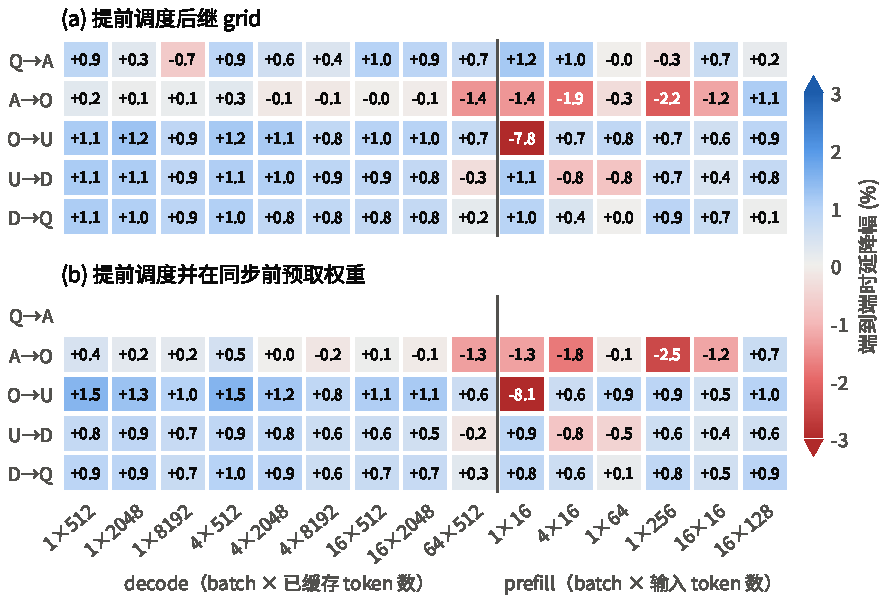
\includegraphics[width=\textwidth]{Img/midterm/pdl_edges}
\caption{五阶段全切分下各类物理边界单独启用 PDL 或带预取 PDL* 相对串行 completion 的端到端时延降幅（正值表示加速）。Q$\to$A 后继为无静态权重的 attention 阶段；色标截断于 $\pm 3\%$，格内标注实测百分比。}\label{fig:pdl}
\end{figure}

\textbf{局限二：借助硬件 PDL 提前启动后继，在异构切分图上并非总能获益。}Hopper 架构提供了硬件级 PDL 机制~\pPDL，允许后继在前驱尚未完全退出时提前启动以隐藏上述间隙。但图~\ref{fig:pdl} 在五阶段全切分上逐边实测的结果表明，PDL 的效果高度分化：decode 中以矩阵为后继的四类边在 36 组仅提前启动测试中有 34 组稳定提速（叠加权重预取最高达 $+1.5\%$）；而在 prefill 中，A$\to$O 边在 5 个负载上均变慢（$-0.3\%$ 至 $-2.2\%$），$1\times 16$ 下的 O$\to$U 边甚至出现 $-7.8\%$ 的明显倒退。在 decode $16\times 2048$ 的全部 31 种切分方案中，对所有物理边界盲目开启 PDL 有 27 种反而慢于纯串行执行。

\subsubsection{边界执行机制的决定因素、相关工作局限与本文思路}\label{sec:factors}

将视野扩展到动态输入规模，如图~\ref{fig:motiv} 所示，15 个覆盖不同 batch 和序列长度的 decode 与 prefill 负载最终分化出 11 种不同的最优逐边执行方案——全图单一 persistent kernel、固定全切分串行、固定全切分全局 PDL 都无法覆盖全部区间。综合上述实测可以清楚地回答问题二：\textbf{一条算子边界应当融合还是切分、切分后是否启用 PDL，由三类可量化的硬件因素共同决定}：
\begin{enumerate}[leftmargin=2.4em,itemsep=2pt]
\item \textbf{两侧阶段的融合资源代价}：融合后因共享寄存器、共享内存和线程块数带来的额外耗时是否高于单次跨 kernel 启动开销（决定该边是融合还是切分）；
\item \textbf{物理边界两侧的共享内存配置兼容性与 SM 剩余资源}：决定 PDL 后继线程块能否顺利提前进入正在执行前驱的 SM，还是被挡在外面、集中挤入最先空闲的少数 SM 引发负载不均；
\item \textbf{后继的 L1 缓存敏感度与前驱尾部的 HBM 带宽余量}：决定提前进入是否因共享内存配置沿用导致 L1 缓存缩水，以及权重预加载是否与前驱争夺 HBM 带宽。
\end{enumerate}

\begin{figure}[!htb]\centering
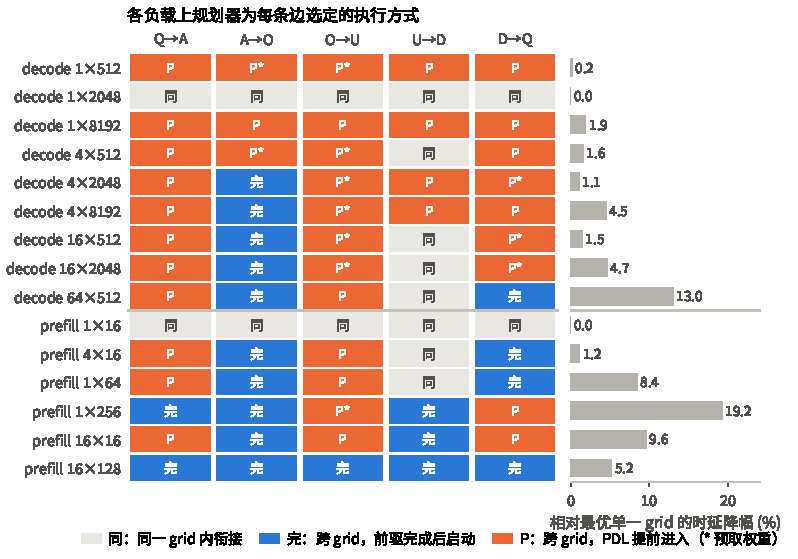
\includegraphics[width=0.9\textwidth]{Img/midterm/motiv_edges}
\caption{15 个典型负载上最优逐边执行方案的分化特征及其相对最优单一 grid 的时延降幅。}\label{fig:motiv}
\end{figure}

对照这三类因素审视现有相关工作，可以看出三点不足：第一，全图单一 kernel 方案（Hazy Megakernels\pHazy、MPK\pMPK）以全融合为既定目标，无法消除异构阶段间的寄存器与共享内存冲突，近期拆解分析~\pQiang 与编译器实践~\pcite{together2026}{Together AI，2026}也证实核内屏障（约 646\,ns）与 CUDA Graph 配合 PDL 的边界开销（约 645\,ns）几乎一致，强行融合反而变慢；第二，现有融合与动态 shape 编译方法多聚焦于单 kernel 内部优化~\pcite{zhengz2022}{Zheng 等，2022a}、静态配置（\rcite{nvidiate}{NVIDIA，2026g}；\rcite{andoorveedu2026}{Andoorveedu 等，2026}）或粗粒度区段切换（\rcite{chatterjee2026}{Chatterjee 等，2026a}；\rcite{chatterjee2026b}{Chatterjee 等，2026b}），而动态 shape 微内核编译如 MikPoly~\pcite{yu2024}{Yu 等，2024} 与 MoonPoly~\pcite{zhangy2026}{Zhang 等，2026a} 仅调节算子内分块参数，算子间仍固定串行启动；第三，在跨 kernel 重叠限制方面，既有记录仅在多流并发下零星观察到共享内存配置干扰（\rcite{nvidiaforum}{NVIDIA，2025}；\rcite{strati2026}{Strati 等，2026}；\rcite{flashinfer7548}{FlashInfer，2026}）或寄存器受限~\pQiang，前期工作 DACOS~\pDacos 也仍以固定算子边界为前提。

因此，本课题的核心思路是：\textbf{不再预设全融合或全切分，而是把阶段图每条边的执行方式提升为决策变量，与各分组的资源配置和硬件调度规律协同求解。}下面两节分别阐述执行机制实现（2.3 节）以及低开销规划与动态 shape 适配方法（2.4 节）。

\subsection{自适应执行机制设计与实现}\label{sec:mech}

围绕问题三，本节首先说明如何在同一套 CUDA 代码上公平实现任意阶段融合与核内分阶段并发控制（2.3.1 节），随后结合前期工作 DACOS 的 PDL 重叠框架剖析 H100 上跨边界重叠的两项底层硬件规律（2.3.2 节），最后导出无需逐边真机试错的静态 PDL 启用规则（2.3.3 节）。

\subsubsection{统一 CUDA 算子实现与核内分阶段并发控制}\label{sec:method}

为了排除外部算子库实现差异、保证不同切分方案在完全一致的算子代码下对比运行，课题实现了一套模板化统一 CUDA 后端：从词嵌入、解码层五个阶段到末层贪心采样共享同一套设备端代码，任意连续阶段区间都可以编译实例化为独立的协作式 persistent grid。具体算子实现上，矩阵阶段提供 $64\times 64$、$128\times 64$ 与 $128\times 16$（列 $\times$ 行）三种 Tensor Core 分块形状，支持沿归约维（K 维）切分，并在收尾融合残差、RMSNorm、RoPE 与 KV 写入；decode attention 采用按历史键值切片并行与双缓冲异步加载的在线归约实现（较早期逐键串行提速 1.1--2.0 倍），prefill attention 同时提供 FlashAttention-2 与零共享内存的逐 warp 在线归约两种实现。

同时，针对多阶段融合在同一个 persistent grid 内时“矩阵偏好 132--264 块、attention 偏好更多块”的内部矛盾，后端引入了\textbf{按物理 SM 重排逻辑块号的核内分阶段活跃块控制}。kernel 启动初期，每个线程块读取硬件寄存器 \texttt{\%smid} 并通过原子计数按“同 SM 内块序号优先、物理 SM 编号次之”重新分配逻辑块号，确保任意前缀子集都能均匀分布到全卡 132 个 SM 上。借此，同一个 persistent kernel 内的矩阵阶段只激活每 SM 1--2 个线程块以保持缓存效率与整波对齐，而 attention 阶段激活全部常驻线程块以充分并行，其余休眠块仅参与轻量屏障同步。实测表明，这一控制让单一 grid 基线自身在 decode $16\times 2048$ 上先提速 6.0\%（由 2201.8\us 降至 2070.8\us），保证了后续所有切分对比都建立在公平的强单核基线之上。

\subsubsection{基于 DACOS 的 PDL 跨边界重叠与 SM 调度规律}\label{sec:pdl}\label{sec:admit}\label{sec:place}

针对物理切分后的算子边界，本课题沿用并拓展了前期已发表工作 DACOS~\pDacos 的依赖感知跨 kernel 重叠框架（图~\ref{fig:dacos}）。DACOS 面向短序列大模型推理中频繁的算子间等待问题，通过三部分机制把相邻 kernel 之间的空闲间隙转化为有效准备与数据预加载：
\begin{enumerate}[leftmargin=2.4em,itemsep=2pt]
\item \textbf{跨 kernel 依赖分析与重叠阶段构造。}对相邻 kernel 依赖边 $(K_i, K_j)$，将后继 $K_j$ 的输入拆分为依赖张量与独立张量，以首次读取依赖张量的同步点——\textbf{依赖前沿} $\mathcal{F}(K_j)$（对应 \texttt{cudaGrid\allowbreak{}Dependency\allowbreak{}Synchronize()}）——为界，把后继拆分为依赖无关的重叠准备阶段与依赖主体 $K_j = K_j^{\mathrm{overlap}} \cup K_j^{\mathrm{dep}}$。其中 $K_j^{\mathrm{overlap}}$ 在前驱尚未结束时即可完成索引与指针计算、张量描述符构建、独立张量向 L2 缓存或共享内存的预加载（如 GEMM 权重预载或 Attention 的 Q 分块预载）及辅助状态初始化。
\item \textbf{三维重叠配置空间与成对代价模型。}前驱 $K_i$ 在可调预启动时机 $\tau_i$ 调用 \texttt{cudaTrigger\allowbreak{}Programmatic\allowbreak{}Launch\allowbreak{}Completion()} 暴露重叠窗口 $W_i(\tau_i)$，后继在由预启动时机 $\tau_i$、预加载数据量 $s_i$ 与存储层级位置 $h_i \in \{\text{L2},\text{SHM},\text{REG}\}$ 构成的配置空间 $\theta_i = \langle \tau_i, s_i, h_i \rangle$ 中择优。DACOS 通过成对代价模型评估重叠执行后的联合时延：
\begin{equation}
\begin{aligned}
\hat{L}_{i,j}(\theta_i) &= T^{\mathrm{base}}(K_i)+T^{\mathrm{dep}}_j+\max\!\bigl(0,\,T^{\mathrm{overlap}}_j(\theta_i)-W_i(\tau_i)\bigr)\\
&\quad -G^{\mathrm{residency}}_i(\theta_i)+P^{\mathrm{cache}}_i(\theta_i),
\end{aligned}
\label{eq:dacos}
\end{equation}
定量权衡超出重叠窗口的未隐藏开销、数据提前驻留收益 $G^{\mathrm{residency}}_i$ 与缓存干扰惩罚 $P^{\mathrm{cache}}_i$。
\item \textbf{参数化模板与运行时实例化。}借助参数化 PDL 内核模板（KPT）和输入形状分桶缓存，DACOS 在运行时为不同输入形状选择最优 $\theta_i^\star$ 并填充启动描述符。在真实短序列 LLM 负载上，DACOS 相对 TorchEager 与 TorchInductor 最高分别取得了 $3.5\times$ 与 $1.2\times$ 的端到端加速。
\end{enumerate}

\begin{figure}[!htb]\centering
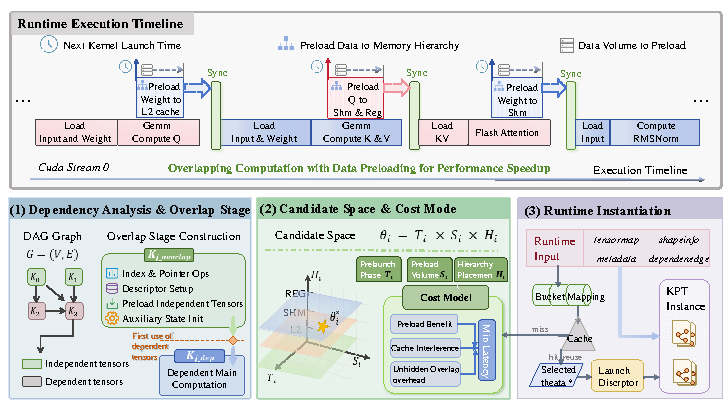
\includegraphics[width=\textwidth]{Img/midterm/dacos_overview}
\caption{前期工作 DACOS~\pDacos 的依赖感知跨 kernel 重叠框架与运行时执行时间线。上方展示在单一 CUDA Stream 中通过 PDL 提前启动后继并将权重/Q 分块预加载至 L2、共享内存或寄存器的重叠过程；下方依次为依赖分析与重叠阶段构造、三维配置空间与代价模型、以及基于形状分桶缓存的运行时实例化流程。}\label{fig:dacos}
\end{figure}

把 DACOS 框架拓展到本课题的可变分组切分图上时，H100 实测进一步揭示了两项此前未被充分刻画的底层硬件限制，正是它们解释了第~\ref{sec:split}~节（图~\ref{fig:pdl}）中部分边开启 PDL 反而变慢的原因：

\textbf{第一，HBM 带宽余量限制了连续矩阵链上的预加载量。}在 H100 受控带宽测试中，如果前驱是不占 HBM 带宽的纯算术负载，仅提前启动后继可省 0.1--0.3\us，叠加 8\,MiB 权重预加载凭借 L2 驻留可将收益放大到 1.0--1.4\us（32--64\,MiB 饱和于 1.5\us）；但当链路是持续打满 HBM 带宽的连续矩阵阶段时，仅提前启动能稳定隐藏 0.4--0.8\us 启动间隙，叠加 1\,MiB 预加载净收益降至 0.2--0.5\us，预加载 8\,MiB 以上则会与前驱抢占 HBM 带宽反而倒退 0.8--7.3\us（真实模型 21 组全切分测试中，1\,MiB 预加载相对纯提前启动的中位变化为 $-0.20$\us 至 $+0.12$\us）。因此，本课题的统一模板将带宽密集链上的重叠前缀限定为轻量初始化与至多 1\,MiB 权重预加载。

\begin{figure}[!htb]\centering
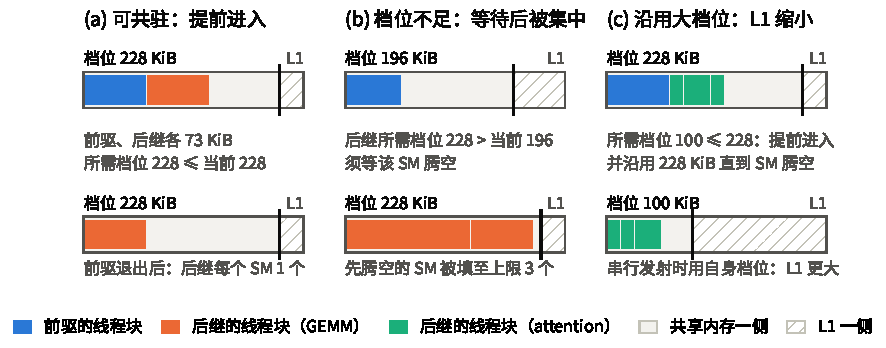
\includegraphics[width=\textwidth]{Img/midterm/v4_carve}
\caption{共享内存 carve-out 配置档位决定的三种 PDL 调度情形。横条表示单个 SM 的统一片上存储，竖线左侧为共享内存、右侧为 L1 缓存：(a) 后继所需档位不高于当前档位且剩余资源充足，顺利提前进入 SM 并发执行；(b) 后继需求档位高于当前档位，被迫等待部分 SM 空闲并集中调度到先空闲的少数 SM；(c) 需求档位较低的后继提前进入后被动沿用前驱大档位，导致可用 L1 缓存容量缩水。}\label{fig:carve}
\end{figure}

\textbf{第二，共享内存配置档位（carve-out）兼容条件决定了 SM 负载均衡。}H100 将单个 SM 的统一片上存储动态切分为共享内存与 L1 缓存，共享内存侧设有 0、8、16、32、64、100、132、164、196 与 228\,KiB 十个离散档位；默认模式下，驱动按“单 SM 最大并发块数 $\times$（单块动态共享内存 $+$ 1\,KiB 系统开销）”向上取整选择最小档位。覆盖 30 组默认档位与 16 组显式档位的微基准证实了两条硬件规则（图~\ref{fig:carve}）：（1）PDL 后继线程块要提前进入仍在执行前驱的 SM，必须同时满足\textbf{所需档位不高于当前生效档位}（显式指定时须严格相等），且该 SM 剩余的共享内存、寄存器与线程槽足以容纳至少一个后继块；（2）SM 当前档位仅在\textbf{该 SM 上全部线程块完全退出后}才会由下一个 kernel 重新配置，而在非空交叠期间会一直沿用。

当后继因档位更高或资源余量不足而无法提前进入非空 SM、且后继总块数又不足以填满全卡所有 SM 槽位时，硬件调度器会把后继线程块集中塞进最先空闲出来的少数 SM 上，引发严重的 \textbf{SM 负载不均}（图~\ref{fig:carve}(b)）。图~\ref{fig:timeline} 展示了真实模型 prefill $1\times 16$（第 2 层）中 O$\to$U 边界的逐块 SM 执行时间线：串行发射下 U 均匀分布于全部 132 个 SM（中位耗时 25.6\us）；仅对该边启用 PDL 时，需求 228\,KiB 档位的 U 无法提前进入低档位前驱 SM，被迫集中挤入先空闲的不到半数 SM（单 SM 挤入 3 块），单阶段耗时增至 33.2\us、整网变慢 9.6\%；而全链连续启用 PDL 使 SM 维持 228\,KiB 高档位时，U 恢复提前进入与均匀分布（26.0\us）。

\begin{figure}[!htb]\centering
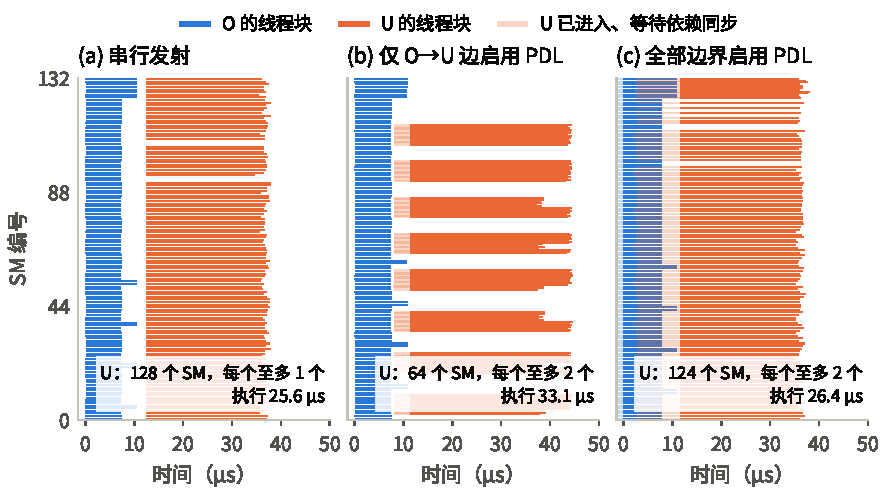
\includegraphics[width=\textwidth]{Img/midterm/v4_timeline}
\caption{真实模型 prefill 1$\times$16（第 2 层）中 O$\to$U 边界在三种模式下的 SM 执行时间线。每条水平线段对应一个线程块的执行起止区间：(a) 串行发射下 U 均匀分布；(b) 仅该边启用 PDL 时 U 因档位不兼容集中落入先空闲的少数 SM；(c) 全链启用 PDL 时 SM 维持高档位，U 恢复提前并发执行且分布均衡。}\label{fig:timeline}
\end{figure}

基于设备端时间戳归纳出的分批均衡派发模型（按约 0.9\us 周期扫描满足档位与余量的候选 SM 并均匀派发待命块），仅利用纯串行运行中记录的前驱退出时刻即可预测 PDL 后继线程块的 SM 分配结果：如表~\ref{tab:place} 所示，在 442 次样本外跨边界发射上，最拥挤 SM 块数的精确命中率达 90\%（两类不可共驻边界分别为 146/146 与 120/124）。受控探针实验（图~\ref{fig:pack}）进一步证实，单 SM 挤入 3 块时实际获取的访存带宽仅为单块 SM 的 1.7 倍，负载不均将尾时延拉长 5.3--7.2\us，与真实模型 7.6\us 的性能退化吻合。

\begin{table}[!htb]\centering
\caption{分批派发模型对 PDL 后继线程块 SM 分配结果的预测精度。命中定义为最拥挤 SM 上的预测后继块数与实测完全一致；SM 数误差给出占用 SM 数绝对偏差的中位数与 90 分位数}\label{tab:place}
\footnotesize\setlength{\tabcolsep}{3.8pt}
\begin{tabular}{@{}lcccccc@{}}
\toprule
 & \multicolumn{3}{c}{基于同次运行退出时刻复现} & \multicolumn{3}{c}{基于串行运行退出时刻样本外预测}\\
\cmidrule(lr){2-4}\cmidrule(l){5-7}
物理边界类别 & 发射次数 & 精确命中 & SM 数误差 & 发射次数 & 精确命中 & SM 数误差\\
\midrule
可提前共驻 SM & 368 & 222（60\%） & 0 / 16 & 172 & 134（78\%） & 0 / 4 \\
不可共驻、后继占满全卡 & 286 & 286（100\%） & 0 / 0 & 146 & 146（100\%） & 0 / 0 \\
不可共驻、后继未占满全卡 & 236 & 225（95\%） & 3 / 44 & 124 & 120（97\%） & 2 / 10 \\
\bottomrule
\end{tabular}
\end{table}

\begin{figure}[!htb]\centering
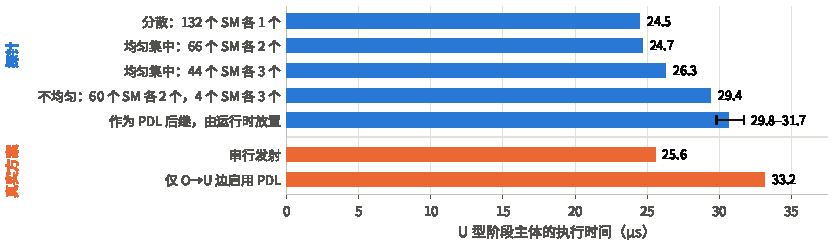
\includegraphics[width=0.94\textwidth]{Img/midterm/v4_pack}
\caption{不同跨 SM 线程块分布对后继执行时间的影响。上图为 U 型矩阵探针（128$\times$16 分块，132 块）在五种空间分布下的耗时，集中调度及真实 PDL 分配显著拉长尾时延；下图对照真实模型 U 阶段在串行与单边 PDL 下的耗时。}\label{fig:pack}
\end{figure}

\subsubsection{L1 缓存容量缩水分析与静态 PDL 启用规则}\label{sec:edge}\label{sec:answer}

除 SM 负载不均外，上述“SM 档位沿执行链保持”的硬件规则还会引发第二类性能退化：\textbf{低共享内存需求的后继如果提前进入高档位前驱 SM，会沿用前驱的大共享内存配置，导致可用的 L1 缓存容量缩水}（图~\ref{fig:carve}(c)）。为了单独量化这一效应，我们在纯串行发射下强制全图采用最大 228\,KiB 共享内存档位进行对照测试（图~\ref{fig:lone}）：显式使用共享内存双缓冲的矩阵阶段几乎不受 L1 容量影响（九成变化在 $\pm 1.4\%$ 以内）；但高度依赖 L1 缓存复用键值数据的 prefill Flash\allowbreak{}Attention-2 变慢 7.3\%--15.5\%，长序列逐 warp attention（$1\times 256$）耗时更由 117\us 飙升至 191\us（增幅 63\%），与全链开启 PDL 时的实测减速一一对应（图~\ref{fig:lone}(b)）。

\begin{figure}[!htb]\centering
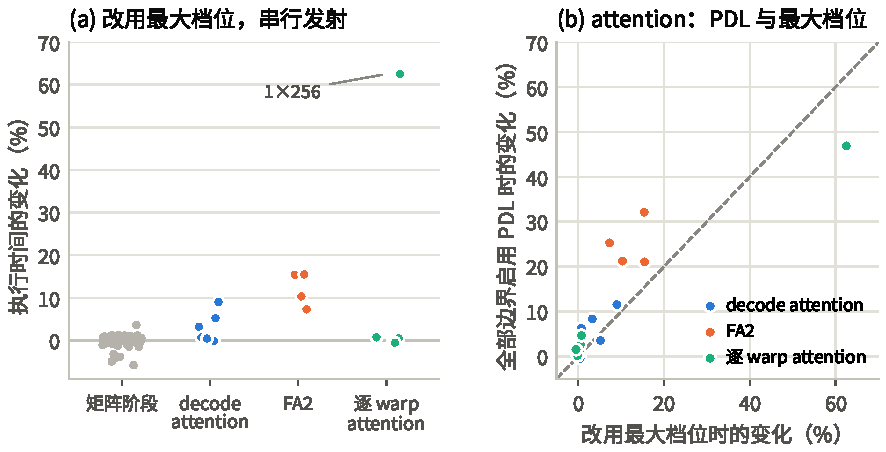
\includegraphics[width=\textwidth]{Img/midterm/v4_l1}
\caption{算子阶段对共享内存 carve-out 档位（剩余 L1 容量）的敏感度差异及其对 PDL 减速的解释。(a) 纯串行发射下强制最大档位引发的各阶段耗时变化；(b) 全链启用 PDL 时 attention 的实际减速幅度与离线测得的 L1 敏感度高度吻合。}\label{fig:lone}
\end{figure}

综合“SM 负载不均”与“L1 缓存缩水”两项硬件机理，仅凭编译期已知的寄存器数、动态共享内存、启动线程块数及对应 carve-out 档位，就可以将任意物理边界静态归入三类：（1）可提前共驻 SM；（2）不可提前共驻但后继线程块占满全卡；（3）不可提前共驻且后继未占满全卡。如图~\ref{fig:cmpdl} 与表~\ref{tab:cmrule} 在 253 类实测物理边界上的检验所示：后继以矩阵阶段开头时，前两类的 113 类边界中有 106 类（94\%）加速、0 类减速（中位数 $+1.0$\us/边），而第三类中有 58\% 减速（最差 $-9.8$\us/边）。由此导出\textbf{基于编译期信息的静态 PDL 启用规则}：
\begin{quote}\small
一条物理边界启用 PDL，当且仅当沿执行链当前生效档位判定该边属于“可提前共驻 SM”或“后继占满全卡”，且若后继以 attention 开头并将沿用更高档位时，其离线测得的 L1 容量缩水代价不超过单次边界节省量（1.0\us）。
\end{quote}
阶段图相邻算子边的完整处理规则汇总于表~\ref{tab:answer}。

\begin{figure}[!htb]\centering
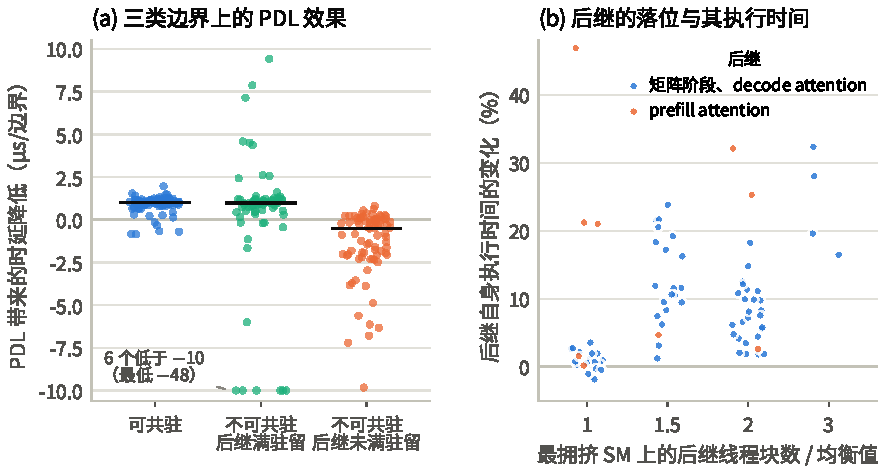
\includegraphics[width=\textwidth]{Img/midterm/v3_pdl}
\caption{物理边界静态三分类对 PDL 实测净收益的区分能力。(a) 253 类边界按静态资源特征分为三类后的单边时延变化分布（横线为中位数）；(b) 16 个全切分方案中后继最拥挤 SM 块数集中程度与后继执行时间增幅的对应关系。}\label{fig:cmpdl}
\end{figure}

\begin{table}[!htb]\centering
\caption{静态三分类在 253 类实测物理边界上的 PDL 单边收益统计（\textmu s/边界，正值表示加速，按后继首阶段类型分列）}\label{tab:cmrule}
\footnotesize\setlength{\tabcolsep}{3.8pt}
\begin{tabular}{@{}llccccccc@{}}
\toprule
静态边界类别 & 后继首阶段 & 样本数 & 中位数 & 四分位区间 & 最差值 & 加速 & 持平 & 减速\\
\midrule
可提前共驻 SM & 矩阵阶段 & 80 & $+1.04$ & $+0.95$ 至 $+1.15$ & $+0.6$ & 80 & 0 & 0 \\
 & Attention & 22 & $+0.58$ & $-0.16$ 至 $+0.89$ & $-0.9$ & 15 & 2 & 5 \\
不可共驻、后继占满全卡 & 矩阵阶段 & 33 & $+1.12$ & $+0.95$ 至 $+2.43$ & $-1.7$ & 26 & 7 & 0 \\
 & Attention & 37 & $+0.69$ & $-0.17$ 至 $+1.07$ & $-47.6$ & 25 & 5 & 7 \\
不可共驻、后继未占满全卡 & 矩阵阶段 & 71 & $-0.89$ & $-2.20$ 至 $+0.03$ & $-9.8$ & 10 & 20 & 41 \\
 & Attention & 10 & $-0.39$ & $-0.80$ 至 $-0.00$ & $-1.4$ & 2 & 1 & 7 \\
\bottomrule
\end{tabular}
\end{table}

\begin{table}[!htb]\centering
\caption{阶段依赖图相邻算子边的处理规则与依据汇总}\label{tab:answer}
\small
\begin{tabularx}{\textwidth}{@{}>{\raggedright\arraybackslash}X>{\raggedright\arraybackslash}p{3.7cm}>{\raggedright\arraybackslash}p{3.2cm}@{}}
\toprule
边界两侧阶段的资源与调度特征 & 选定边处理方式 & 支撑依据\\
\midrule
两侧资源需求接近，融合执行无额外损失（如单请求短上下文 decode、极短序列逐 warp prefill） & 保留同 grid 融合（配合核内分阶段活跃块控制） & 表~\ref{tab:cores}，表~\ref{tab:decode}\\
一侧需更高线程块并发、占满寄存器预算或偏好不同分块，融合资源损失高于单次启动开销 & 切分为物理边界，两侧分组独立配置分块与块数 & 表~\ref{tab:cores}，图~\ref{fig:rule}\\
已切分物理边界；后继可提前共驻 SM 或已占满全卡，且无超阈值 L1 缩水代价 & 启用跨 grid PDL（后继含静态权重且有带宽余量时可预载 1\,MiB） & 表~\ref{tab:cmrule}，图~\ref{fig:rulereal}\\
已切分物理边界；后继不可提前共驻且未占满全卡（易引发先空闲 SM 上的集中调度） & 采用跨 grid completion 串行执行 & 图~\ref{fig:timeline}，表~\ref{tab:cmrule}\\
已切分物理边界；后继为 L1 敏感的 attention 且提前进入将沿用高档位 & 采用跨 grid completion 串行执行 & 图~\ref{fig:lone}，图~\ref{fig:rulereal}\\
\bottomrule
\end{tabularx}
\end{table}

\subsection{划分方案搜索与动态 Shape 自适应框架}\label{sec:search_sys}\label{sec:sys}

有了执行机制和静态 PDL 规则后，本节回答问题四：面临庞大的分组切分与参数配置组合，如何在不逐点真机穷举的前提下快速构造高质量划分方案？当线上请求 batch 与序列长度动态变化时，又该如何低开销地切换执行计划？

\subsubsection{基于线程块波次的分组耗时解析模型}\label{sec:cm}

要避免每次改变输入规模都在真机上遍历上百组配置，核心在于建立足够准确、又能跨配置泛化的分组耗时解析模型。我们自底向上拆解矩阵与 attention 阶段的执行耗时：

在\textbf{矩阵主循环层面}，权重常驻 L2 时的部件消融实验（图~\ref{fig:ablate}）表明，小分块主循环主要受片上异步装载通路限制：$128\times 16$ 与 $64\times 64$ 分块剥离异步拷贝可缩短每步耗时 28\%--41\%，明显大于剥离 MMA 计算指令的 18\%--26\%；每 SM 并发 3 块时，纯异步拷贝甚至因装载通路饱和而反慢于完整循环。当权重需从 HBM 流式读取时（图~\ref{fig:cmloop}），每步耗时随并发读取的相异权重块数迅速触及 2.96\,TB/s 带宽上限，随输入行数 $M$ 增大则借助行方向权重复用平滑过渡到计算主循环受限。

\begin{figure}[!htb]\centering
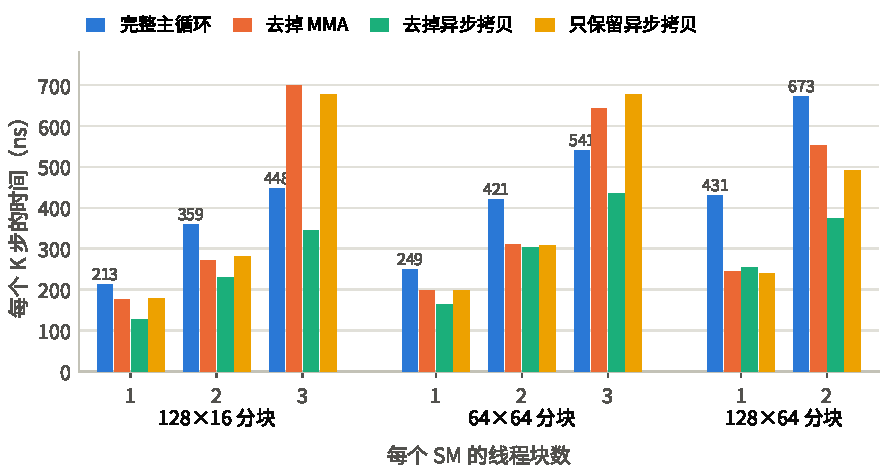
\includegraphics[width=0.95\textwidth]{Img/midterm/v4_ablate}
\caption{矩阵主循环部件消融实验（权重常驻 L2 时单个 K 步耗时）。小分块下剥离异步拷贝节省的时间显著高于剥离 MMA 指令；每 SM 并发 3 块时纯异步拷贝因装载通路过载反慢于完整循环。}\label{fig:ablate}
\end{figure}

\begin{figure}[!htb]\centering
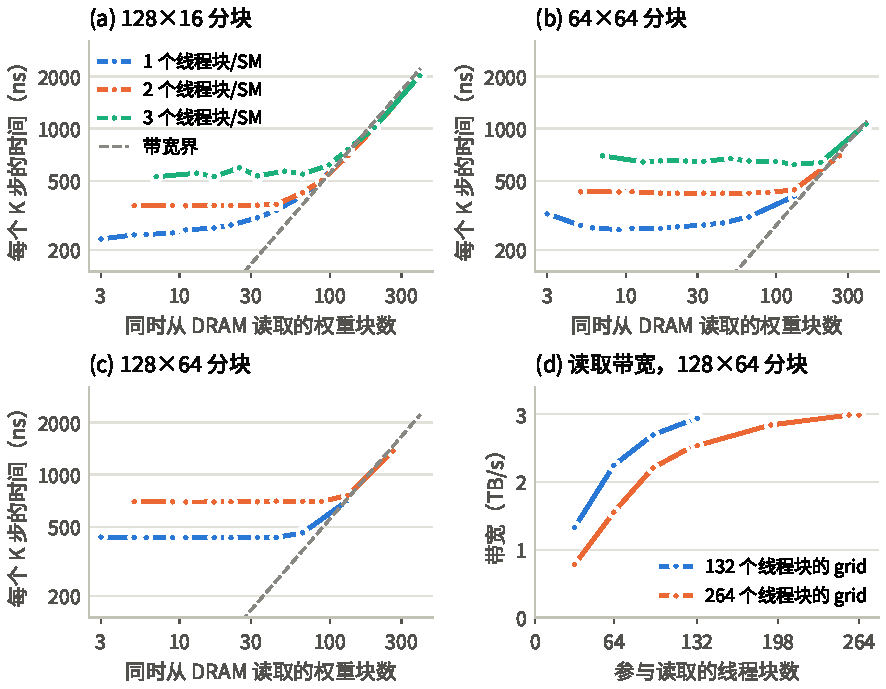
\includegraphics[width=0.94\textwidth]{Img/midterm/v3_loop}
\caption{片外流式读取下每个 K 步耗时向 HBM 带宽上限的过渡规律。(a)--(c) 三种分块形状下每步耗时随并发读取相异权重块数的变化（虚线为 2.96\,TB/s 带宽界）；(d) 128$\times$64 分块下有效读取带宽随参与线程块数的变化。}\label{fig:cmloop}
\end{figure}

在\textbf{完整单阶段层面}，扫描 1 至 2048 行的 43 个行数（共 1376 个测点）可以清晰看到由线程块波次（wave quantization）主导的阶梯曲线（图~\ref{fig:cmladder}）：每当行数越过分块行数整数倍导致总波数 $W$ 加一，耗时就会阶跃上升（如 U 阶段从 128 行的 32.0\us 跨入 129 行第二波时跃升至 47.0\us，增幅 47\%）。结合核内计时分解（表~\ref{tab:cmtl}），矩阵阶段总耗时可解析表达为固定开销、多波主循环与尾部逐元素第二遍三项之和：
\begin{equation}
T=T_{\mathrm{fix}}+\sum_{w=1}^{W}\bigl[t_{\mathrm{wave}}(n_w,c_w,k)+t_{\mathrm{epi}}\bigr]+T_{\mathrm{2nd}}, \label{eq:stage}
\end{equation}
其中波数 $W$、第 $w$ 波新读权重块数 $n_w$、单 SM 参与块数 $c_w$ 与单任务 K 步数 $k$ 均由分块映射直接算得；完全复用微探针常数而不实测真实阶段的为模型 A（留出中位误差 3.9\%），仅在 16、64、2048 三个采样行数标定尾部系数的为模型 B（留出中位误差 3.4\%）。

\begin{figure}[!htb]\centering
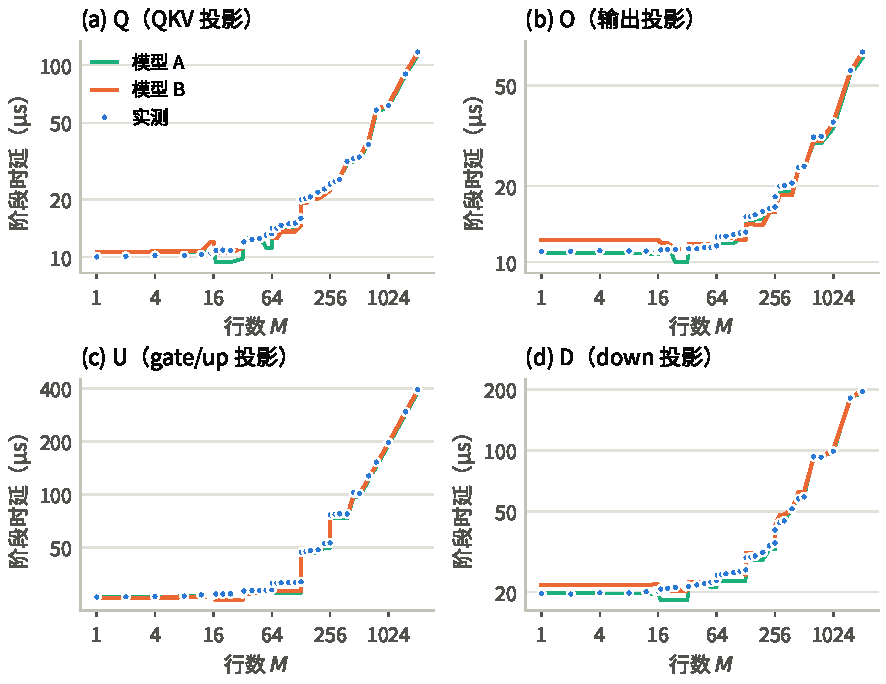
\includegraphics[width=\textwidth]{Img/midterm/v3_ladder}
\caption{四个矩阵阶段独立成组时随输入行数的波次阶梯曲线及解析模型拟合效果。模型 A 完全复用微探针常数，模型 B 仅使用 16、64 与 2048 三个采样行数标定尾部系数，均准确复现了其余 40 个留出行数上的台阶位置与幅值。}\label{fig:cmladder}
\end{figure}

\begin{table}[!htb]\centering
\caption{矩阵阶段独立成组时核内各组成部分的实测耗时分解（\textmu s，取对应行数最优分块/块数配置）}\label{tab:cmtl}
\footnotesize\setlength{\tabcolsep}{4.2pt}
\begin{tabular}{@{}lrlccrrrrrr@{}}
\toprule
阶段 & 行数 & 最优配置 & \makecell{K 维\\切分} & 波数 & \makecell[r]{固定\\开销} & \makecell[r]{主循\\环遍} & \makecell[r]{核内\\屏障} & \makecell[r]{尾部第\\二遍} & 计时合计 & 生产实测\\
\midrule
Q & 16 & 128$\times$16 / 264 & 8 & 1 & 2.2 & 6.6 & 1.2 & 1.0 & 11.0 & 10.8 \\
Q & 256 & 64$\times$64 / 396 & 2 & 1 & 2.3 & 13.3 & 1.5 & 6.0 & 23.2 & 23.6 \\
Q & 2048 & 128$\times$64 / 264 & 1 & 3 & 2.3 & 71.2 & 1.2 & 40.8 & 115.6 & 116.9 \\
O & 16 & 128$\times$16 / 132 & 8 & 1 & 2.1 & 4.7 & 1.2 & 3.5 & 11.7 & 11.2 \\
O & 256 & 64$\times$64 / 264 & 2 & 1 & 2.2 & 9.1 & 1.7 & 3.1 & 16.3 & 16.5 \\
O & 2048 & 128$\times$64 / 264 & 1 & 2 & 2.2 & 49.9 & 1.1 & 14.5 & 67.8 & 67.9 \\
U & 16 & 128$\times$16 / 132 & 1 & 1 & 2.3 & 24.3 & -- & -- & 26.8 & 27.0 \\
U & 256 & 128$\times$64 / 264 & 1 & 2 & 2.2 & 50.6 & -- & -- & 53.0 & 53.1 \\
U & 2048 & 128$\times$64 / 264 & 1 & 16 & 2.2 & 388.7 & -- & -- & 391.0 & 394.1 \\
D & 16 & 128$\times$16 / 132 & 8 & 1 & 2.2 & 12.8 & 1.2 & 3.8 & 20.1 & 20.3 \\
D & 256 & 128$\times$64 / 264 & 4 & 1 & 2.2 & 26.8 & 1.3 & 4.2 & 34.7 & 35.0 \\
D & 2048 & 128$\times$64 / 264 & 1 & 2 & 2.2 & 180.1 & 1.1 & 16.3 & 199.7 & 195.9 \\
\bottomrule
\end{tabular}
\end{table}

进一步发现，当每 SM 并发 3 个线程块时，同 SM 内三个线程块之间稳定存在 17\% 的速度差异（14.6\us 至 17.1\us），而整波完成时间由最慢的那一块决定。将单波时长 $t_{\mathrm{wave}}$ 由中位数修正为同 SM 最慢线程块耗时后，模型 A 在每 SM 3 块下的留出中位误差由 10.9\% 降至 3.8\%（图~\ref{fig:order}，模型 B 为 3.5\%）。连同按最重工作单元建立的三种 attention 参数化模型，单阶段留出集精度汇总于表~\ref{tab:cm_all_acc}（矩阵阶段仅实测模型推荐的前 2 个配置即可将相对最优的平均性能损失压至 0.34\%）。

在\textbf{多阶段融合分组层面}，任意连续多阶段分组 $g$ 的耗时无需新增组合拟合参数，直接由固定开销、各阶段主体耗时与核内屏障线性相加得到：
\begin{equation}
T_g=T_{\mathrm{fix}}+\sum_{s\in g}B_s(x,\theta_g)+(|g|-1)\,t_{\mathrm{bar}}. \label{eq:group}
\end{equation}
在真实模型采集的全部 2177 组配置上检验（图~\ref{fig:group} 与表~\ref{tab:group}），整体中位误差仅为 4.9\%，其中纯矩阵多阶段分组误差（2.9\%--3.5\%）与单阶段基本持平；仅含高寄存器 FlashAttention-2 的融合分组因跨阶段指令相互干扰误差偏高（15.3\%），将作为下一阶段模型精细化的重点。

\begin{figure}[!htb]\centering
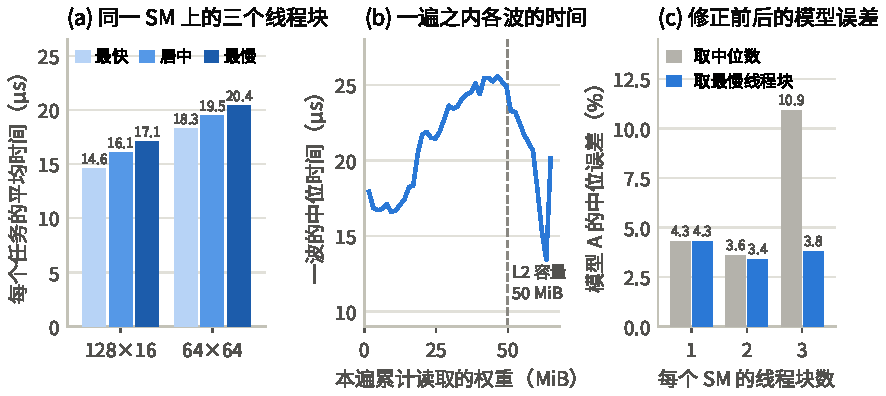
\includegraphics[width=0.95\textwidth]{Img/midterm/v4_order}
\caption{高并发密度下同 SM 线程块的速度差异及其对模型精度的修正效果。(a) 每 SM 并发 3 块时同 SM 内快、中、慢三个线程块的单任务耗时差异；(b) 多波推进过程中随累计权重逼近 L2 容量出现的单波耗时抬升；(c) 改按最慢线程块建模前后在三种并发密度下的留出集中位误差对比。}\label{fig:order}
\end{figure}

\begin{table}[!htb]\centering
\caption{单阶段解析模型（模型 B）在留出测试集上的时延预测误差与配置选择精度}\label{tab:cm_all_acc}
\footnotesize\setlength{\tabcolsep}{4.2pt}
\begin{tabular}{@{}llccccc@{}}
\toprule
阶段类型 & 评估对象 & \makecell{检验\\测点数} & \makecell{中位误\\差（\%）} & \makecell{90 分位\\误差（\%）} & \makecell{命中实测\\最优比例} & \makecell{相对最优平\\均损失（\%）}\\
\midrule
矩阵阶段 & Q 阶段 & 320 & 3.2 & 8.9 & \multirow{4}{*}{140/160（Top-2）} & \multirow{4}{*}{0.34（Top-1: 1.39）} \\
 & O 阶段 & 320 & 4.1 & 10.7 &  &  \\
 & U 阶段 & 320 & 3.4 & 10.7 &  &  \\
 & D 阶段 & 320 & 2.9 & 8.1 &  &  \\
 & 四阶段汇总 & 1280 & 3.4 & 10.0 & 140/160 & 0.34 \\
\midrule
Attention & Decode 切片归约 & 100 & 5.1 & 15.8 & 14/25（Top-1） & 3.70 \\
 & Prefill，FA2 & 28 & 6.5 & 19.8 & 14/14（Top-1） & 0.00 \\
 & Prefill，逐 warp & 56 & 12.1 & 21.2 & 13/14（Top-1） & 0.10 \\
\bottomrule
\end{tabular}
\end{table}

\begin{figure}[!htb]\centering
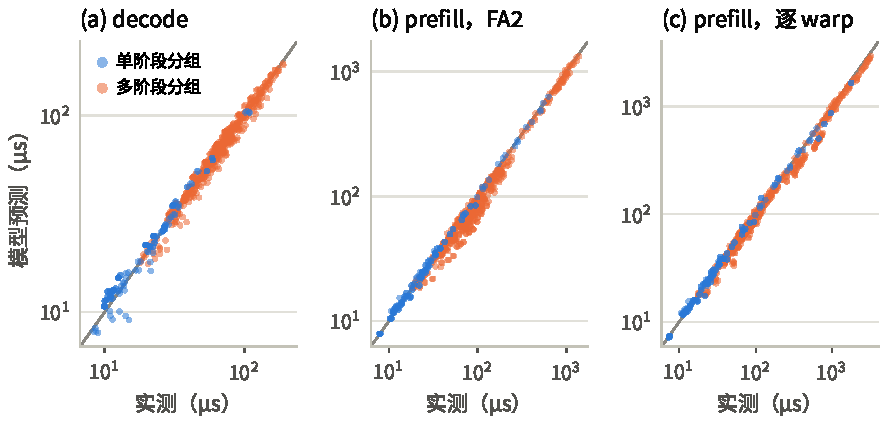
\includegraphics[width=0.94\textwidth]{Img/midterm/v3_group}
\caption{零组合拟合参数下多阶段分组模型预测值与真实模型 2177 组实测耗时的对比散点图（不含首尾词嵌入与词表投影分组）。}\label{fig:group}
\end{figure}

\begin{table}[!htb]\centering
\caption{分组时延模型在 2177 组真实模型配置上的相对误差分布（\%，报告中位数与 90 分位数）}\label{tab:group}
\footnotesize\setlength{\tabcolsep}{4.5pt}
\begin{tabular}{@{}lccccccccc@{}}
\toprule
 & & \multicolumn{2}{c}{全部配置} & \multicolumn{2}{c}{单阶段分组} & \multicolumn{2}{c}{\makecell{多阶段分组\\（不含 attention）}} & \multicolumn{2}{c}{\makecell{多阶段分组\\（含 attention）}}\\
\cmidrule(lr){3-4}\cmidrule(lr){5-6}\cmidrule(lr){7-8}\cmidrule(l){9-10}
阶段与实现 & 配置总数 & 中位 & 90 分位 & 中位 & 90 分位 & 中位 & 90 分位 & 中位 & 90 分位\\
\midrule
Decode & 731 & 4.1 & 12.7 & 7.8 & 16.0 & 3.5 & 11.8 & 4.0 & 11.5 \\
Prefill，FA2 & 672 & 5.8 & 23.7 & 2.7 & 9.4 & 2.9 & 9.0 & 15.3 & 30.7 \\
Prefill，逐 warp & 774 & 5.2 & 16.3 & 3.3 & 10.9 & 3.0 & 8.9 & 8.0 & 23.5 \\
\bottomrule
\end{tabular}
\end{table}

\subsubsection{模型与静态规则引导的离线规划方法}\label{sec:search}\label{sec:guided}

在没有代价模型和静态规则辅助时，基准穷举规划器需要在每个输入规模上遍历全部多阶段分组配置、端到端实测全部 32 种切分方案并逐边贪心搜索 PDL 开关，单负载耗时达 35--262\,s。结合式~(\ref{eq:group}) 的分组耗时模型与第~\ref{sec:edge}~节的静态 PDL 启用规则，课题将其压缩为紧凑的\textbf{四步引导式离线规划流程}：
\begin{enumerate}[leftmargin=2.4em,itemsep=2pt]
\item \textbf{分组配置筛选}：对不含首尾层的多阶段分组直接按式~(\ref{eq:group}) 排序并仅实测排名第一的配置；单阶段分组扫描基准块数，并为 attention 加测一次最大共享内存档位以标定其 L1 缩水代价；
\item \textbf{切分拓扑粗排}：以各分组最优耗时之和减去静态规则核准的 PDL 预计节省量（按 1.0\us/边计）为 31 种切分方案快速打分，仅截取前 6 名进入端到端实测候选；
\item \textbf{PDL 规则生成}：取消逐边贪心试探，直接为入围切分方案生成静态规则集合、附带 1\,MiB 权重预载集合、链式档位一致集合与全开对照（每拓扑至多 4 个变体）；
\item \textbf{端到端定案}：在选择集上将上述候选与最优单一 grid 实测对比，输出最终计划。
\end{enumerate}
该流程在几乎不损失端到端性能的前提下将真机测量量大幅削减（具体评测见第~\ref{sec:exp}~节）。

\subsubsection{动态 Shape 决策分类与离线—在线协同架构}\label{sec:types}\label{sec:arch}

要处理线上推理中 batch 和序列长度的动态变化，不可能在每次前向推理时重新运行规划器，必须搞清楚执行计划 $\Pi=\langle C,\{\theta_g\},\{\varphi_e\}\rangle$ 中哪些决策可以离线写死、哪些必须随输入规模调整。为此，我们在 15 个代表负载上全量采集了单一 grid 与 31 种切分方案（累计 1649 个端到端方案）的交替重放时延，以“将某项决策固定后，在全部负载上最多会慢多少”为衡量标准，在 1.0\% 容差内将执行计划划分为三类：
\begin{enumerate}[leftmargin=2.4em,itemsep=2pt]
\item \textbf{固定型决策（离线固化）。}如图~\ref{fig:types}(a) 所示，同属矩阵阶段、资源需求一致的 U$\to$D 边在全部负载上固定融合的最大损失不超过 0.3\%；decode 阶段其余四条边统一固定为切分（即 Q|A|O|UD 分组）跨全负载最大损失也仅 0.6\%。
\item \textbf{切换型决策（仅保留两种机制候选）。}prefill 阶段除 U$\to$D 外的四条边随融合代价由负转正同步切换（图~\ref{fig:types}(b)）。因此切分层无需保留全部 32 种拓扑，只保留\textbf{“全模型单一 grid”和“Q|A|O|UD 四边切分”两个候选}（图~\ref{fig:types}(c)），即可将跨负载切分损失压在 0.6\% 以内（无先验自动选两项也仅 1.4\%）；而各物理边界的 PDL 开关由静态规则直接导出，在 Q|A|O|UD 上相对串行稳定提速 0.8\%--4.2\%。
\item \textbf{参数型决策（按有效行数分区间建表）。}与切分方式高度收敛相反，各分组的分块形状与线程块数随输入行数高频变化（图~\ref{fig:tile}）：43 个扫描行数上四个矩阵阶段经历 5--16 次切换，固定单一配置的最大损失高达 16\%--22\%（decode attention 固定 528 块最大损失达 26\%）。不过，在 1\% 容差内合并相邻最优配置相同的行数后，覆盖全部行数只需约 22 个有效行数区间（5\% 容差下缩至 15 个区间）。
\end{enumerate}

\begin{figure}[!htb]\centering
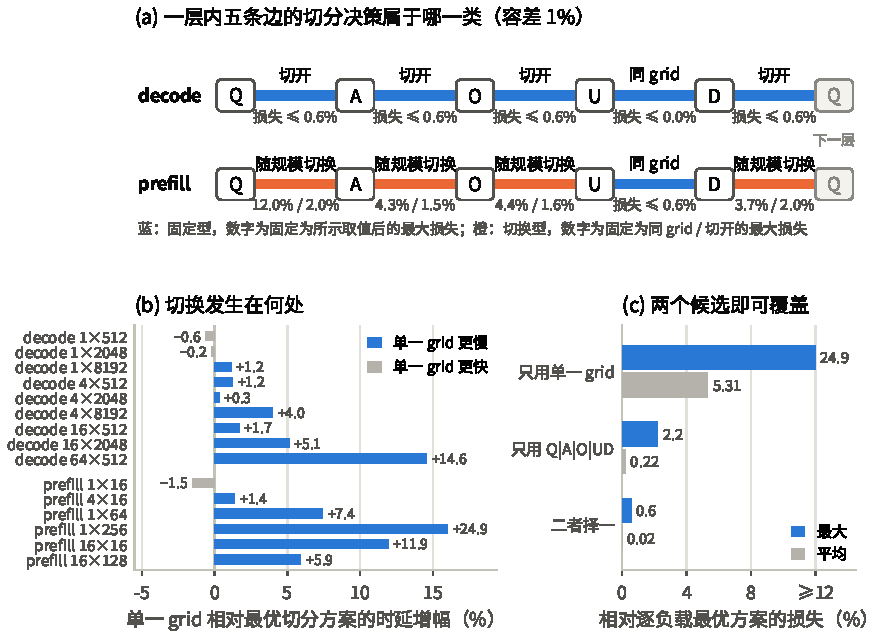
\includegraphics[width=\textwidth]{Img/midterm/v5_colour}
\caption{容差 1\% 下五类算子边切分决策的敏感度分类与候选压缩效果。(a) Decode 与 prefill 阶段各边切分决策所属类别及固定后的最大相对时延损失；(b) 各负载下单一 grid 相对最优切分方案的时延增幅；(c) 切分层仅保留单一候选或双候选集合时的跨负载最大与平均损失。}\label{fig:types}
\end{figure}

\begin{figure}[!htb]\centering
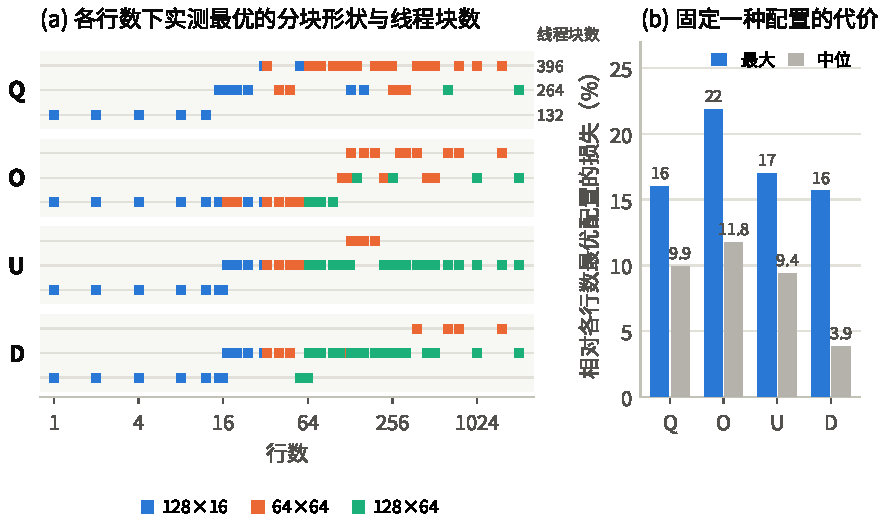
\includegraphics[width=\textwidth]{Img/midterm/v5_tile}
\caption{分组资源配置沿输入行数轴的参数型跳变特征。(a) 四个矩阵阶段在 43 个行数上实测最优的分块形状与启动线程块数；(b) 全局固定采用单一配置（128$\times$64 分块、264 个线程块）相对逐行数最优配置的时延损失。}\label{fig:tile}
\end{figure}

基于上述三类划分，课题确立了如图~\ref{fig:arch} 所示的\textbf{“离线准备—在线选择”两阶段系统架构}：离线阶段（每个模型与目标 GPU 只执行一次）完成统一后端编译、模型与静态规则引导规划、决策分类，并按有效行数区间组织双候选执行方案、分组资源配置及预捕获 CUDA Graph 候选计划表；在线阶段（每次前向推理）根据实时请求的 batch 和序列长度算出有效行数，查表取出对应计划并更新运行参数直接重放，保证候选表规模线性可控且在线路径零搜索。目前离线侧候选生成、引导规划与 15 负载决策分类已完成，二维全网格计划表与在线查表执行器将在下一阶段（2027.01–04）落地实现。

\begin{figure}[!htb]\centering
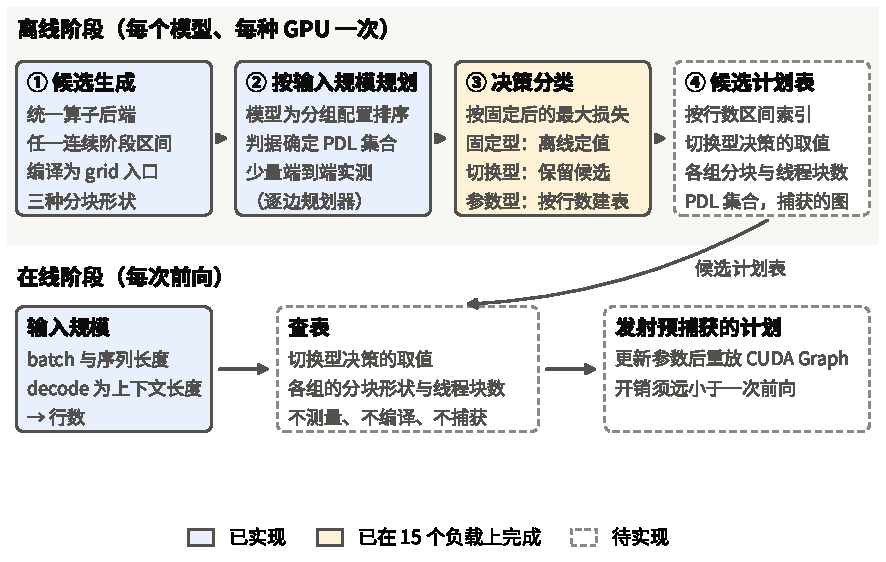
\includegraphics[width=\textwidth]{Img/midterm/v5_arch}
\caption{面向动态输入规模的“离线准备—在线选择”两阶段系统架构。离线阶段一次性完成统一算子编译、模型与规则引导规划、规模敏感度分类及候选计划表构建；在线阶段根据实时请求有效行数直接查表重放预捕获 CUDA Graph。}\label{fig:arch}
\end{figure}

\subsection{阶段性实验评估与分析}\label{sec:exp}

本节在真实模型权重与英文文本语料上，依次评估上述自适应执行机制的端到端性能收益、静态 PDL 规则的可靠性以及模型引导规划器的搜索效率。

\subsubsection{实验环境与评测设置}

全部实验在单张 NVIDIA H100 80GB HBM3 GPU（132 个 SM，CUDA 12.3）上基于 Llama-3.2-1B-Instruct 的 BF16 权重执行，覆盖 9 组 decode 负载（batch $\times$ 缓存上下文长度）与 6 组 prefill 负载（batch $\times$ 输入序列长度）。真实语料严格切分为互不重叠的选择集与报告集：规划搜索仅使用选择集，最终时延与 95\% 分块自助法置信区间均在报告集上经 CUDA Graph 捕获后通过 20 个随机乱序测量块交替重放获取。所有参评方案均通过严格数值正确性检查：贪心采样输出与 Hugging Face 参考实现完全一致，logits KL 散度不超过 0.02，新写入 KV 缓存相对二范数误差不超过 4\%。对比基线分为四类：（1）全阶段统一线程块数的“统一配置单一 grid”；（2）加入逻辑块重排与核内分阶段活跃块控制的“最优单一 grid”；（3）固定全切分串行与全局开启 PDL 方案；（4）主流外部推理系统 vLLM~\pVllm 与 Mirage MPK~\pMPK。

\subsubsection{端到端性能收益与对比分析}

表~\ref{tab:decode} 与表~\ref{tab:prefill} 汇总了 15 个基准负载上的端到端评测结果，图~\ref{fig:gain} 展示了不同机制对端到端加速的逐层贡献：
\begin{itemize}[leftmargin=2.0em,itemsep=2pt]
\item \textbf{Decode 阶段（表~\ref{tab:decode}）：}规划器在 8 个负载上选出含物理切分与逐边 PDL 的方案（主要收敛至 Q|A|O|UD 与全切分，仅 $1\times 2048$ 保留单一 grid），相对最优单一 grid 缩短单步时延 0--13.0\%（相对统一配置单一 grid 缩短 0.1\%--13.0\%）。按贡献来源拆解（图~\ref{fig:gain}(a)）：核内分阶段活跃块控制先为单核基线消除最高 6.0\% 内部并发失配；物理切分使 attention 突破 396 块上限扩展至 528 块，在 $4\times 8192$、$16\times 2048$ 与 $64\times 512$ 上直接贡献最高 11.6\% 降幅；逐边 PDL 进一步削减 1.6\%--5.4\% 算子间等待间隙，使原本单纯切分变慢的中小批量负载（$1\times 8192$、$4\times 512$、$16\times 512$）转为正收益。相比之下，固定全切分串行（$-5.4\%$ 至 $+10.4\%$）与全局开启 PDL（$-1.7\%$ 至 $+7.1\%$）均在多个工作点性能退化。
\item \textbf{Prefill 阶段（表~\ref{tab:prefill}）：}相对取较快 attention 实现的最强单一 grid 基线，规划方案缩短首 token 时延 0--19.2\%（图~\ref{fig:gain}(b)）。序列长度 16 的单请求负载由逐 warp 单核即达最优（1352.5\us），而 $16\times 16$ 因矩阵与 attention 偏好不同配置仍获 9.61\% 降幅；序列长度增至 64 及以上后，物理切分将占满 255 寄存器的 FlashAttention-2 隔离至独立 kernel，使相邻矩阵分组恢复每 SM 3 块并发，在 $1\times 64$、$1\times 256$ 与 $16\times 128$ 上分别取得 8.43\%、19.23\% 与 5.21\% 加速。
\item \textbf{收益规律与外部系统对比：}将 15 个负载的端到端收益与 16 层累计共驻代价占比对照（图~\ref{fig:rule}），二者 Spearman 秩相关系数达 $\rho=0.92$：累计共驻代价占比超 8\% 的 7 个负载仅凭切分即获超 4.5\% 加速；其余 8 个低代价负载中，6 个靠逐边 PDL 获 0.2\%--1.95\% 正收益，2 个自动保留单一 grid。横向对比主流外部系统，规划方案在全部 decode 与中小规模 prefill 负载上较 vLLM~\pVllm 分别缩短时延 25\%--41\% 与 41\%--71\%，在单请求负载（decode $1\times 512$、prefill $1\times 16$ 与 $1\times 64$）上较 Mirage MPK~\pMPK 分别提速 21\%、33\% 与 79\%。
\end{itemize}

\begin{table}[!htb]\centering
\caption{Decode 阶段端到端单步时延（\textmu s）及规划方案相对两级单一 grid 基线的时延降幅（\%）}\label{tab:decode}
\small
\begin{tabular}{@{}lrrrrr@{}}
\toprule
测试负载 & \makecell[r]{统一配置\\单一 grid} & \makecell[r]{最优\\单一 grid} & 规划方案 & \makecell[r]{相对统一配置\\降幅（\%）} & \makecell[r]{相对最优单一 grid 降幅\\及 95\% 置信区间（\%）}\\
\midrule
1$\times$512 & 1368.5 & 1366.8 & 1364.1 & $+0.3$ & $+0.19$ [0.17, 0.24] \\
1$\times$2048 & 1439.5 & 1438.0 & 1438.0 & $+0.1$ & 0 \\
1$\times$8192 & 1640.4 & 1628.8 & 1597.1 & $+2.6$ & $+1.95$ [1.54, 2.09] \\
4$\times$512 & 1428.7 & 1428.2 & 1405.1 & $+1.7$ & $+1.62$ [1.34, 1.74] \\
4$\times$2048 & 1604.3 & 1562.5 & 1545.7 & $+3.6$ & $+1.07$ [1.02, 1.12] \\
4$\times$8192 & 2137.9 & 2030.3 & 1938.8 & $+9.3$ & $+4.50$ [4.43, 4.58] \\
16$\times$512 & 1681.8 & 1616.4 & 1592.4 & $+5.3$ & $+1.49$ [1.34, 1.64] \\
16$\times$2048 & 2201.8 & 2070.8 & 1974.4 & $+10.3$ & $+4.65$ [4.52, 4.79] \\
64$\times$512 & 2514.6 & 2514.4 & 2187.0 & $+13.0$ & $+13.02$ [12.97, 13.12] \\
\bottomrule
\end{tabular}
\end{table}

\begin{table}[!htb]\centering
\caption{Prefill 阶段首 token 时延（\textmu s）及规划方案相对最优单一 grid（取两种 attention 实现中较快者）的降幅（\%）}\label{tab:prefill}
\footnotesize\setlength{\tabcolsep}{5.2pt}
\begin{tabular}{@{}lrrrrr@{}}
\toprule
 & \multicolumn{2}{c}{最优单一 grid 时延} & \multicolumn{2}{c}{规划方案时延} & \\
\cmidrule(lr){2-3}\cmidrule(lr){4-5}
测试负载 & FlashAttention-2 & 逐 warp & FlashAttention-2 & 逐 warp & \makecell[r]{相对最优基线降幅\\及 95\% 置信区间}\\
\midrule
1$\times$16 & 1587.5 & \textbf{1352.5} & 1489.0 & \textbf{1352.5} & 0 \\
4$\times$16 & 1798.7 & \textbf{1587.1} & 1659.6 & \textbf{1568.6} & $+1.17$ [0.99, 1.29] \\
1$\times$64 & \textbf{1779.4} & 1780.9 & \textbf{1629.5} & 1780.9 & $+8.43$ [8.14, 8.60] \\
1$\times$256 & \textbf{3161.1} & 5979.1 & \textbf{2553.3} & 4199.2 & $+19.23$ [19.09, 19.41] \\
16$\times$16 & 3020.6 & \textbf{2895.1} & 2642.3 & \textbf{2617.0} & $+9.61$ [9.50, 9.73] \\
16$\times$128 & \textbf{14670.4} & 26919.6 & \textbf{13906.4} & 21402.0 & $+5.21$ [4.43, 5.56] \\
\bottomrule
\end{tabular}
\end{table}

\begin{figure}[!htb]\centering
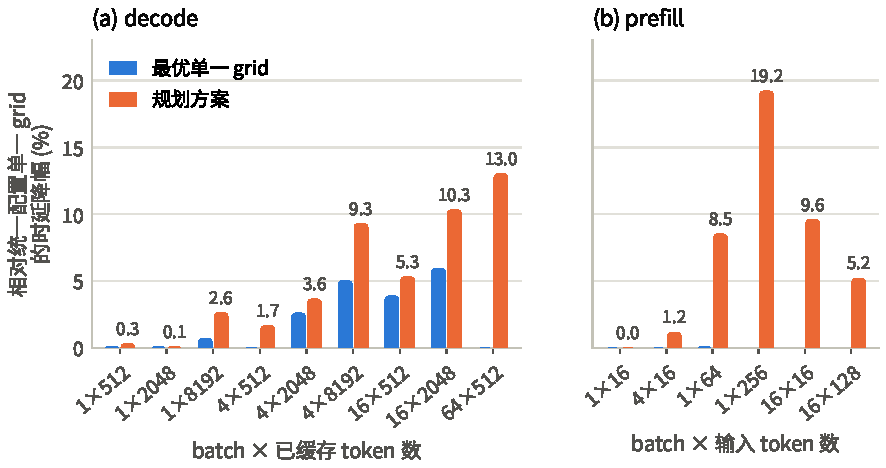
\includegraphics[width=\textwidth]{Img/midterm/gain}
\caption{15 个基准负载上最优单一 grid 与规划方案相对统一配置单一 grid 的端到端时延降幅对比。柱顶数字标注规划方案的总降幅，清晰区分核内分阶段活跃块控制与物理切分/PDL 各自的贡献。}\label{fig:gain}
\end{figure}

\begin{figure}[!htb]\centering
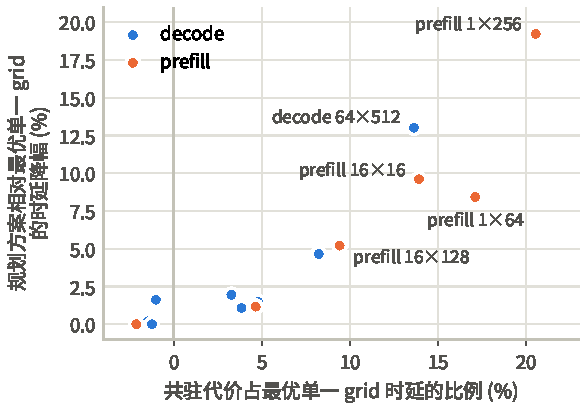
\includegraphics[width=0.66\textwidth]{Img/midterm/rule}
\caption{全网累计共驻代价占比与规划方案端到端收益的定量相关性（Spearman 秩相关系数 $\rho=0.92$）。}\label{fig:rule}
\end{figure}

\subsubsection{PDL 静态规则与引导式规划器验证}

首先检验静态 PDL 启用规则的端到端效果。在微观层面，decode $1\times 512$ 全切分五类边界的核内计时分解表明，PDL 将算子间等待间隙由 1.95--2.21\us 压缩至 0.67--0.78\us，扣除后继轻微负载不均增加的 0.4--0.8\us 后，每条边界净节省 0.58--0.80\us。在全部 16 组真实全切分方案上对比三种 PDL 策略（图~\ref{fig:rulereal}）：全局盲目开启导致 10 个方案慢于串行（最差 $-18.8\%$，中位数 $-0.45\%$）；本文提出的静态 PDL 规则在全部 16 组方案上实现零负向回退，中位加速 $+1.98\%$，与逐边实测贪心搜索（$+1.71\%$）相当。

\begin{figure}[!htb]\centering
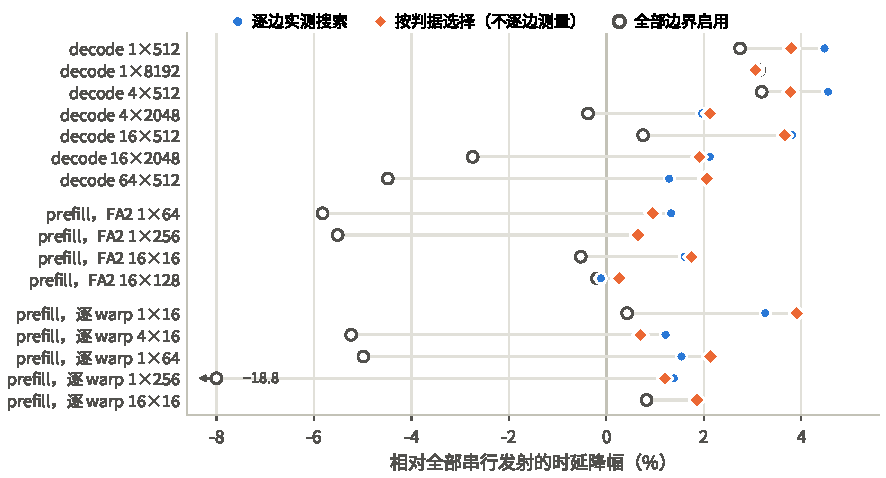
\includegraphics[width=\textwidth]{Img/midterm/v4_rulereal}
\caption{16 个真实模型全切分方案上三种 PDL 策略相对纯串行 completion 的端到端时延降幅对比。静态 PDL 规则在全部方案上均无负收益，整体表现与逐边实测搜索相当。}\label{fig:rulereal}
\end{figure}

其次检验模型与静态规则引导的离线规划器。图~\ref{fig:guided} 在全部 15 个基准负载上对比了引导式规划器与基准穷举规划器的测量开销与方案质量：引导式流程将分组配置实测次数压缩至穷举的 62\%、整网端到端实测次数压缩至 20\%，总测量量降至 43\%（单负载中位规划耗时由 40\,s 缩短至 21\,s，prefill $16\times 128$ 由 262\,s 降至 99\,s）；同时，报告集上的端到端时延偏差严格控制在 $\pm 1.0\%$ 以内（中位数 $-0.15\%$，峰值加速 19.6\%），验证了受控搜索空间规划的高效性与可靠性。

\begin{figure}[!htb]\centering
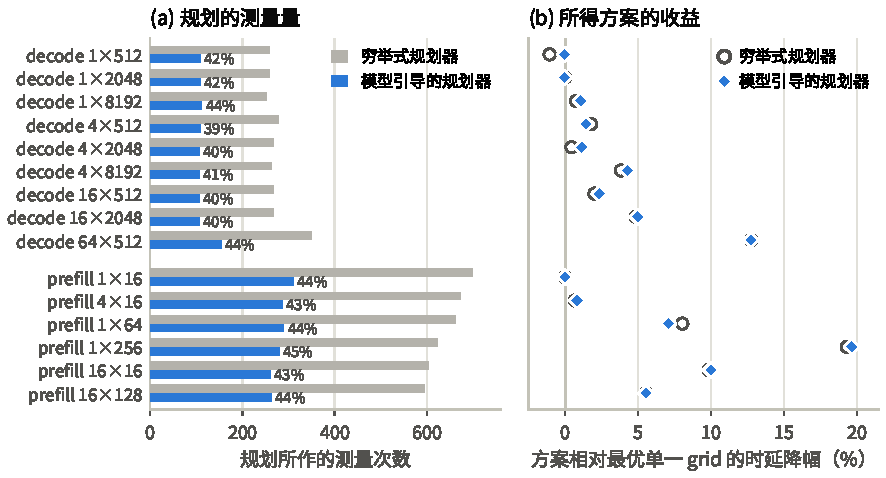
\includegraphics[width=\textwidth]{Img/midterm/v4_guided}
\caption{模型与静态规则引导规划器相对穷举规划器的测量开销缩减与端到端收益保持度。(a) 15 个基准负载上的总实测次数对比（条末百分比为引导式占穷举式的比例）；(b) 两种规划器选出方案在报告集上相对最优单一 grid 的时延降幅。}\label{fig:guided}
\end{figure}


\section{下一步工作计划和内容}
\subsection{现存问题与下一步工作内容}

对照开题确立的完整系统目标，当前工作已完成机理分析、解析建模与离线引导规划，但在四方面仍需进一步深化：其一，面向任意计算图的前端 lowering 模块，以及含高寄存器 FlashAttention-2 融合分组和首尾层分组的代价模型精度尚待完善；其二，面向动态 shape 的决策敏感度分类、“离线准备—在线选择”两阶段调度架构及二维“batch $\times$ 序列长度”输入网格候选计划表尚未开展系统实现；其三，第四项研究内容（完整框架实现与端到端连续 token 生成验证）尚未开启，核内细粒度事件与大矩阵异步流水亦有待并入；其四，跨层异构分组、7B/8B 等更大模型规模及多卡张量并行中的通信节点边处理尚待拓展。

围绕上述问题，后续研究沿两条线索推进：一方面，收尾第一阶段工作 DACOS~\pDacos，将其在短序列大模型上的方法与面向通用网络及多流依赖选择的扩展整理为期刊论文；另一方面，按以下四项任务推进第二阶段完整系统构建与验证：
\begin{enumerate}[leftmargin=2.4em,itemsep=3pt]
\item \textbf{解析代价模型精细化与前端依赖模块封装。}改进含 FlashAttention-2 融合分组的寄存器占用建模与核内分阶段活跃块控制修正项，补齐首尾词嵌入与词表投影分组模型；将 attention 的 L1 敏感度建模为序列长度的连续函数并将共享内存档位纳入配置空间；独立封装面向通用计算图的前端依赖分析与 lowering 模块，在留出行数与非整倍分块边界测点上验证模型精度。

\item \textbf{面向动态 Shape 的离线—在线自适应调度机制与执行器实现。}正式开启第四项研究内容，研究 batch 与序列长度动态变化下执行计划的决策敏感度分类（区分可离线固定的决策、随规模切换的少量机制候选与按有效行数区间索引的资源参数），构建覆盖“batch $\times$ 序列长度”二维网格、共享权重与激活缓冲池的预捕获 CUDA Graph 候选计划表及在线查表调度器，定量评估表项规模、显存占用、预热耗时与区间切换开销；并放宽各层同构约束，探索跨层异构边处理的收益空间。

\item \textbf{多卡张量并行中集合通信节点的边处理扩展。}探索将分布式推理中 AllReduce 等集合通信作为图节点纳入统一边级决策空间：在双卡张量并行配置下构建通信节点与相邻计算阶段的候选衔接方式，量化为通信预留 SM 对相邻矩阵波次划分与 PDL 共享内存配置档位的影响，明确通信连边在动态输入规模下的决策类别（不涉及底层通信路由算法设计）。

\item \textbf{完整框架端到端验证与跨规模性能评估。}将局部就绪边上的核内细粒度事件并入统一后端，引入 Hopper 异步 TMA/WGMMA 流水优化大矩阵主循环并压缩 Q 阶段尾部访存开销；完成多步连续自回归 token 生成的端到端集成，在 1B 及 7B/8B 等不同参数规模模型和动态请求负载上系统报告 TTFT、TPOT、P50/P90/P99 分位数时延与全模块消融分析。
\end{enumerate}

\subsection{进度安排}

后续各阶段的工作重点与可验收阶段成果如表~\ref{tab:next} 所示，整体时间节点与开题报告保持一致。

\begin{table}[!htb]\centering
\caption{后续研究工作进度与可验收成果安排}\label{tab:next}
\small
\begin{tabularx}{\textwidth}{@{}>{\raggedright\arraybackslash}p{2.4cm}>{\raggedright\arraybackslash}p{2.1cm}>{\raggedright\arraybackslash}X>{\raggedright\arraybackslash}p{4.1cm}@{}}
\toprule
时间节点 & 对应任务 & 主要研究工作 & 可验收阶段成果\\
\midrule
2026.12 & 前期收尾、任务一 & 完成 DACOS 期刊扩展稿撰写；改进含 attention 融合及首尾层分组的代价模型，封装通用前端依赖分析模块 & 期刊投稿稿件；留出行数及分块边界上模型配置选择的误差评估报告\\
2027.01–2027.02 & 任务二、任务四 & 启动框架实现与端到端验证，完成动态 shape 决策分类、二维输入网格候选计划表与在线查表执行器；并入核内细粒度事件并完成连续 token 生成集成 & 可运行的自适应推理框架原型；计划表规模—显存—切换开销与端到端正确性验证报告\\
2027.03–2027.04 & 任务三、任务四 & 在动态负载与连续生成场景下开展跨 batch、上下文与模型规模（含 7B/8B）评测及系统消融；完成双卡通信节点边处理实验 & 跨模型规模 TTFT、TPOT 与分位数结果；双卡通信边处理对比与完整消融数据\\
2027.05–2027.06 & 总结与论文撰写 & 完善系统源码与可复现实验包，撰写第二阶段学术论文与硕士学位论文，准备学位论文答辩 & 完整系统原型与复现材料；第二阶段学术论文稿件与硕士学位论文\\
\bottomrule
\end{tabularx}
\end{table}

\subsection{预计答辩时间}

按照上述研究进度安排，预计于 2027 年 5 月至 6 月完成硕士学位论文撰写与答辩工作。


\section{已取得科研成果列表}
\begin{enumerate}
  \item 郝朝阳等. DACOS: Dependency-Aware Cross-Kernel Overlapping for Optimizing Short-Sequence Workloads in LLM Applications. 未发表稿\cite{hao2026dacos}。
\end{enumerate}


\section*{参考文献}
\addcontentsline{toc}{section}{参考文献}
{\sloppy\small\linespread{1.35}\selectfont
\begin{list}{}{\setlength{\leftmargin}{2em}\setlength{\itemindent}{-2em}\setlength{\itemsep}{3pt}\setlength{\parsep}{0pt}}
\refitem{cheng2026} Cheng X, Zhang Z, Zhou Y, et al. MPK: A compiler and runtime for mega-kernelizing tensor programs [C/OL]//20th USENIX Symposium on Operating Systems Design and Implementation (OSDI 26). Seattle, WA: USENIX Association, 2026: 1909-1926. \url{https://www.usenix.org/conference/osdi26/presentation/cheng}.
\refitem{dao2024} Dao T. Flashattention-2: Faster attention with better parallelism and work partitioning [C]//The Twelfth International Conference on Learning Representations. 2024.
\refitem{hao2026} Hao Z, Li G, Luo F, et al. DACOS: Dependency-Aware Cross-Kernel Overlapping for Optimizing Short-Sequence Workloads in LLM Applications [C]//European Conference on Parallel Processing (Euro-Par 2026), Lecture Notes in Computer Science. 2026: 409-422.
\refitem{hazy2025b} Hazy Research. Megakernels: Low-latency LLM inference with device-side task graphs [EB/OL]. 2025[2026-07-20]. \url{https://github.com/HazyResearch/Megakernels/tree/7309cec801537b61fea3b50d7dfe454a6cde578e}.
\refitem{kwon2023} Kwon W, Li Z, Zhuang S, et al. Efficient memory management for large language model serving with PagedAttention [C/OL]//Proceedings of the 29th Symposium on Operating Systems Principles. 2023: 611-626. DOI: 10.1145/3600006.3613165.
\refitem{nvidia2026a} NVIDIA. CUDA programming guide 13.3: CUDA graphs [EB/OL]. 2026[2026-07-20]. \url{https://docs.nvidia.com/cuda/cuda-programming-guide/04-special-topics/cuda-graphs.html}.
\refitem{nvidia2026b} NVIDIA. CUDA programming guide 13.3: Programmatic dependent launch and synchronization [EB/OL]. 2026[2026-07-20]. \url{https://docs.nvidia.com/cuda/cuda-programming-guide/}.
\refitem{spector2025} Spector B, Juravsky J, Sul S, et al. Look ma, no bubbles! Designing a low-latency megakernel for Llama-1B [EB/OL]. Hazy Research Blog, 2025. \url{https://hazyresearch.stanford.edu/blog/2025-05-27-no-bubbles}.
\end{list}\par}
\clearpage

\section*{附录\quad 相关研究进展}
\addcontentsline{toc}{section}{附录\quad 相关研究进展}

本课题围绕动态负载下计算图的逐边执行机制选择展开：对计算图上的每一条连边，决定相邻两个计算阶段是在同一 persistent grid 内衔接、拆分为两次独立 launch 并按完成语义（completion）串行推进，还是在拆分边界上借助 Programmatic Dependent Launch（PDL）使后继提前进入并与前驱重叠；同时联合决定与之耦合的分组级资源配置（线程块数、分块形状、共享内存与寄存器预算）。当输入规模动态变化时，上述边界机制与资源配置的最优组合亦随之改变。围绕这一核心问题，近年文献可归纳为十三条研究线索：驻留式执行的演进与早期反思、大模型推理中的全图驻留执行、执行边界与后端的联合决策、融合编译器中的边界判据、动态 shape 与负载自适应优化、跨 kernel 重叠机制、kernel 内分工与跨 kernel 空间划分、GPU 片上资源共享的体系结构研究、分块与波量化（wave quantization）、性能代价模型、通信—计算重叠边、智能体驱动的 kernel 自动生成，以及推理服务系统与高性能算子库基线。其中前八条线索主要刻画执行形态的演进，后续线索则聚焦给定执行形态下的参数寻优与判据建模。

\subsubsection*{一、驻留式执行的演进与全图融合的固有代价}

将多个计算阶段放入单个长期驻留的 kernel 并非全新范式。\rcite{gupta2012}{Gupta 等 (2012)} 较早系统总结了 persistent threads 编程模型，通过启动恰好填满设备驻留容量的线程块并在设备端循环拉取任务，规避主机侧逐次 launch 开销及硬件调度器的不可控性。\rcite{steinberger2014}{Steinberger 等 (2014)} 提出的 Whippletree 在此基础上构建了面向动态异构任务的设备端调度框架。进入深度学习领域后，\rcite{diamos2016}{Diamos 等 (2016)} 的 Persistent RNN 将循环层权重常驻于片上存储以消除时间步间的重复访存，\rcite{holmes2019}{Holmes 等 (2019)} 的 GRNN 进一步将该思路拓展至低时延 RNN 推理。细粒度设备端运行时亦沿此路线演进：\rcite{yeh2017}{Yeh 等 (2017)} 的 Pagoda 利用常驻 MasterKernel 虚拟化 GPU 资源，按 warp 粒度调度并行度不足的窄任务，相对 CUDA Hyper-Q 取得平均 1.51$\times$ 加速；\rcite{belviranli2018}{Belviranli 等 (2018)} 的 Juggler 则在设备端完成依赖解析与任务派发，避免粗粒度全局屏障同步，在科学计算负载上相对全局屏障方案最高提升 31\%。

然而，“将完整计算图无条件融进单一 megakernel”在图形学领域很早便被证实存在固有代价。\rcite{laine2013}{Laine 等 (2013)} 在波前路径追踪研究中明确指出，单一 megakernel 的寄存器分配上限受其中资源需求最苛刻的阶段支配，其余轻量阶段被迫在同一低占用率（occupancy）约束下运行；将其拆分为若干独立阶段 kernel 并在阶段间重排任务反而显著更快。这一机理与本课题在 H100 上观测到的现象高度一致：单一 persistent kernel 的共享内存 carve-out 档位与每线程寄存器预算完全由最重阶段（如占用 255 个寄存器的 FlashAttention-2）决定，从而压低其余矩阵阶段的驻留上限。本课题在早期构建上的对照实验表明，当将 decode 阶段的 attention 从 255 寄存器实现替换为 91 寄存器实现后，物理切分相对最优单一 grid 的收益便由 14.4\%--16.5\% 收缩至 $-2.3\%$ 到 $+8.0\%$，印证了相当一部分切分收益源自解除重阶段对共驻代码的资源拖累。与路径追踪中动态数据驱动队列不同，大语言模型推理各阶段之间具有确定的数据依赖图结构，因而能够以算子边为单位精细权衡共驻与切分。

在深度学习编译器方向，\rcite{ma2020}{Ma 等 (2020)} 的 Rammer 提出 rTask 与 vEU 抽象，将算子内与算子间并行纳入同一静态调度空间并在 persistent kernel 中执行；\rcite{zhuang2024}{Zhuang 等 (2024)} 的 MonoNN 进一步将完整推理网络编译为单体 kernel，以发掘逐算子优化无法触及的跨阶段复用空间。这两项工作均将单一 kernel 视为既定终态，调度自由度仅存在于 kernel 内部，物理边界本身并非决策变量。与之互补，\cGraph 通过将多 kernel 序列固化为可重放有向无环图来摊销主机侧提交代价，但默认依赖边仍遵循“上游完全结束—下游方才启动”的串行完成语义。

\subsubsection*{二、大模型推理中的全图驻留执行}

近两年来，全图驻留式 megakernel 在低时延 LLM 推理领域得到集中推进。\rcite{spector2025}{Spector 等 (2025b)}（Hazy Research）面向 Llama-1B 手工构建了设备端任务图解释器，利用细粒度原子计数器替代全 grid 屏障维护跨阶段依赖，成为公开单请求 decode 时延最低的实现之一（本课题在 H100 上实测其 $B{=}1, S{=}512$ 单步时延为 1.08\,ms）。\rcite{he2026}{He 等 (2026)} 的 VDCores 针对异步 GPU 架构提出资源与执行解耦的编程模型；\cMPK 将设备端任务图方法系统编译器化，自动将张量程序降低为 SM 级任务与事件图并扩展至多卡通信场景，报告相对传统服务系统最高取得 1.7$\times$ 的端到端时延收益；\rcite{jin2026}{Jin 等 (2026)} 的 Event Tensor 则将分块任务间的依赖关系提升为一等张量抽象，通过编译器 ETC 联合实施静态与动态调度变换以支持动态 shape，并重点优化了固定形态 megakernel 在在线服务中的编译预热开销。

围绕上述主干路线近期出现了三方面扩展。其一是受限片上资源下的精细管理：\rcite{dong2026}{Dong 等 (2026)} 的 Ada-MK 针对消费级/推理级架构严格的共享内存与寄存器限制，借助 MLIR 细粒度依赖分解与离线静态轨迹搜索固化执行计划，并通过共享内存分页复用在在线广告推理场景中稳定超越 TensorRT-LLM。其二是基于智能体的自动代码合成：\rcite{li2026f}{Li 等 (2026a)} 的 ForgeMegakernel 结合里程碑知识库与中间态校验预言机自动生成 decode megakernel，在 0.6B--13B 模型上报告了相对 SGLang 平均 1.21$\times$、相对 MPK 平均 1.54$\times$ 的加速；\rcite{jaber2026}{Jaber 和 Jaber (2026)} 的 AutoMegaKernel 引入静态调度 IR 验证器以在启动前排除死锁与数据竞争，但也坦陈在 A100/H100 上受跨 SM 同步开销制约，部分场景仍慢于经 CUDA Graph 封装的 cuBLAS。其三是面向异构计算—通信混合负载的核内空间划分：\rcite{huang2026}{Huang 等 (2026a)} 的 Weave 与 \rcite{mao2026}{Mao 等 (2026)} 的 mKernel 在单核或跨机融合 kernel 内部将 SM 动态划分为计算组与通信组，分别在多卡 MoE 与 Ring Attention 等负载上取得显著重叠收益。此外，\rcite{yangy2026}{Yang 等 (2026)} 的 GPUOS 探索向运行中的常驻 kernel 动态注入即时编译算子，\rcite{chowdhary2026}{Chowdhary 等 (2026)} 的 Fleet 引入面向多芯粒（multi-die）GPU 的局部 L2 亲和任务层级，而 \rcite{guo2026}{Guo 和 Miao (2026)} 的 PipeLink 则利用资源契约静态检验加载、主循环与收尾组件能否安全链接进同一 kernel。

总体来看，这一方向仍普遍以单一驻留 kernel 作为默认目标形态，将优化重心放在 kernel 内部的 SM 角色划分与事件同步上，因而未能从根本上摆脱异构阶段共驻时的包络木桶效应。

\subsubsection*{三、执行边界与后端的联合决策}

近期若干前沿工作开始正面审视“在哪里切分 megakernel”这一问题。\cChat 将流式推理模型的分段切分显式建模为连续区段划分、区段后端选择（常规算子图或 megakernel）及跨区段共享策略的三元组搜索，依托独立算子剖析与排序代理评分免去端到端遍历，发现 NH-TTS、Qwen3-TTS 与 Llama-1B 上的最优方案随 batch 规模在零至四个 megakernel 之间动态迁移；\rcite{chatterjee2026b}{Chatterjee 等 (2026b)} 进一步在连续批处理迭代边界上根据实时并发度在整图 megakernel 与常规融合链之间二选一，在 128 并发与 8 并发区间分别兼顾了高吞吐与低时延。

与此同时，\cQiang 从微观机制层给出了极具启发性的实证反思。该工作基于同一份底层算子代码将 ThunderKittens 与 VDCores 两个代表性 megakernel 拆解重构为独立 kernel 序列，证实线程块常驻并不天然等价于有效计算重叠：配合 PDL 重叠启动与权重加载后，拆分版 ThunderKittens 的 decode 时延反而降低 5.7\%。作者通过细粒度插桩指出，设备端细粒度发布与内存序维护本身存在可观开销，在途异步访存流量较高时信号发布时延显著上升；更重要的是，persistent 线程块可在内部直接复用片上存储，而分离 launch 的后继 kernel 必须在 SM 上获取完整的线程块资源配额后方能准入执行。不过，该文将这一准入限制归结为对未来 GPU 细粒度跨核资源共享硬件支持的诉求，尚未在现有硬件上提炼出可定量预测的准入判据。本课题前期工作 DACOS（\cDacos）则从固定算子边界出发，在合法性约束下联合决策后继预启动时机、操作数预取规模与存储层级放置。

此外，相邻方向还在空间流水与编译搜索层面展开了探索：\rcite{andoorveedu2026}{Andoorveedu 等 (2026)} 的 SubGPU Pipelining 与 \rcite{davies2025}{Davies 等 (2025)} 的 Kitsune 将计算图切分为绑定于互斥 SM 子集的空间流水段；\rcite{dai2025}{Dai 等 (2025)} 的 STOF 与 \rcite{huangz2026f}{Huang 等 (2026b)} 的 FlashFuser 联合搜索算子融合边界与分块流水配置；\rcite{lix2026}{Li 等 (2026c)} 的 AgentCompile 在四档离散融合粒度间择优；\rcite{linj2026}{Lin 等 (2026b)} 的 MegaOps 则在保持 kernel 分离的前提下将依赖粒度下沉至单个中间分块。在工业界实践中，NVIDIA Transformer Engine 的 Userbuffers 后端（\rcite{nvidiate}{NVIDIA, 2026g}）、CoCoNet（\rcite{jangda2022}{Jangda 等, 2022}）与 PyTorch async-TP（\rcite{wangy2024}{Wang 等, 2024}）已支持逐算子静态配置重叠策略；\rcite{together2026}{Together AI (2026)} 的工程报告更直接指出，H100 上 megakernel 内部全局同步（约 646\,ns）与 CUDA Graph 配合 PDL 的跨边界交接（约 645\,ns）开销几乎一致，迫使全图统一 warp 数与 cluster 规模反而带来显著减速，因此转而为模型各条边手工标注同步方式。

对比可见，现有工作或以粗粒度区段与整次前向为单位切换后端，或仅在离线初始化阶段静态指定重叠策略，尚未将“同 grid 共驻、跨 grid completion 与跨 grid PDL”作为逐边决策变量与分组级资源配置联合求解，亦缺乏在现役硬件上直接判定 PDL 准入与落位代价的解析依据。

\subsubsection*{四、融合编译器中的边界判据}

传统深度学习图编译器围绕算子融合边界积累了四类代表性判据。第一类是基于算子属性分类的启发式规则，如 TVM（\rcite{chen2018}{Chen 等, 2018}）、Ansor（\rcite{zhengl2020}{Zheng 等, 2020}）、DNNFusion（\rcite{niu2021}{Niu 等, 2021}）与 Hidet（\rcite{ding2023}{Ding 等, 2023}）。第二类是基于访存流量与并行度衰减的解析代价模型，如基于 tile-graph 的 Welder（\rcite{shi2023}{Shi 等, 2023}）、Chimera（\rcite{zhengs2023}{Zheng 等, 2023}）、MCFuser（\rcite{zhangzh2024}{Zhang 等, 2024}）及分层反馈融合框架 Apollo（\rcite{zhao2022}{Zhao 等, 2022}）。第三类是精确数学规划或超优化枚举，如将原语重组表述为 0-1 线性规划的 Korch（\rcite{hu2024}{Hu 等, 2024}）与多级超优化器 Mirage（\rcite{wu2025}{Wu 等, 2025}）。第四类则如 Triton（\rcite{tillet2019}{Tillet 等, 2019}）与 TileLang（\rcite{wangl2025}{Wang 等, 2025}），由程序员显式界定 kernel 范围而由编译器优化内部流水。

上述工作中有两项设计与本课题密切相关。一方面，片上驻留资源上限已被引入融合切分判据：例如 Souffle（\rcite{xia2024}{Xia 等, 2024}）要求子程序内部全局同步所需的最大占用不超过单波驻留容量，超限即切分为新 kernel；AStitch（\rcite{zhengz2022}{Zheng 等, 2022a}）则根据共享内存与寄存器压力在寄存器、共享内存和全局内存多级缝合方式间降级。但这些判据仅检验单个融合组自身的驻留合法性，并未刻画相邻两个独立 kernel 能否在同一 SM 上跨边界交叠驻留。另一方面，AStitch 与 Welder 虽支持逐边选择数据复用层级，但其候选操作均局限于同一 kernel 内部，并未纳入“保留物理边界并利用硬件 PDL 抵消交接开销”这一跨边界维度。

\subsubsection*{五、动态 shape 与负载自适应优化}

真实推理服务中请求到达率、提示长度与缓存上下文持续波动，使面向动态 shape 的编译优化成为本课题系统设计的重要参照。该领域的经典架构普遍遵循“离线构建候选空间、在线轻量匹配”的分工模式：Nimble（\rcite{shen2021}{Shen 等, 2021}）、DISC（\rcite{zhu2021}{Zhu 等, 2021}）与 BladeDISC（\rcite{zhengz2024}{Zheng 等, 2024a}）在编译期保留符号化维度关系；DietCode（\rcite{zhengb2022}{Zheng 等, 2022b}）、MikPoly（\rcite{yu2024}{Yu 等, 2024}）与 MoonPoly（\rcite{zhangy2026}{Zhang 等, 2026a}）离线生成固定尺寸微内核并在运行时依实际输入规模动态拼合；FlashDecoding++（\rcite{hong2024}{Hong 等, 2024}）、WaveTune（\rcite{zhang2026}{Zhang 等, 2026b}）与 DeepGEMM（\rcite{deepgemm2025}{DeepSeek, 2025a}）则根据矩阵形状动态切换算子内部的分块配置或数据流。

然而，上述动态 shape 编译器与算子库在运行时调整的对象均限于单个算子内部的分块参数与微内核组合，算子间始终固定为逐 kernel 串行启动；而前述 megakernel 自适应工作（\cChat；\rcite{chatterjee2026b}{Chatterjee 等, 2026b}；\rcite{wu2026}{Wu 等, 2026}；\rcite{yadav2026}{Yadav 和 Zhao, 2026}）又仅在整段或整次前向粒度上切换后端。本课题的跨负载实验（正文图~\ref{fig:motiv} 与第~\ref{sec:types}~节）表明，在无约束逐负载寻优下 15 个典型负载会产生 11 种不同的逐边方案；而进一步引入 1\% 时延容差作敏感度解耦后可以发现，边级切分机制在 decode 上可离线固定、在 prefill 上仅需两个协同候选即可覆盖，真正沿行数轴频繁更替的是各分组的分块形状与线程块配置（约需 22 个行数区间）。这一认识将动态 shape 自适应自然推广至“少量机制候选 + 分段资源配置查表”的联合空间。

\subsubsection*{六、跨 kernel 重叠执行机制}

作为 Hopper 架构引入的硬件级跨边界协同原语，PDL 允许前驱通过 \texttt{griddepcontrol.launch\_dependents} 提前释放后继调度资格，并由后继在首次依赖读取前通过 \texttt{cudaGridDependencySynchronize}（对应 PTX 指令 \texttt{griddepcontrol.wait}）保证数据可见性（\cPDL）。当前主流推理框架（如 SGLang 的低时延模式）多将 PDL 视为全局开关对前向链近乎全量开启；而 Hazy Megakernels（\rcite{spector2025}{Spector 等, 2025b}）则认为其同步粒度偏粗而完全退回单核内部同步。此外，SET（\rcite{li2026s}{Li 等, 2026b}）、Blink（\rcite{siavashi2026}{Siavashi 等, 2026a}）、设备端多卡任务图（\rcite{mustard2025}{Turimbetov 等, 2025}）以及体系结构层的 Wireframe（\rcite{wireframe2017}{Abdolrashidi 等, 2017}）与 BlockMaestro（\rcite{blockmaestro2021}{Abdolrashidi 等, 2021}）分别从流事件图重用、网卡/设备端自驱动与硬件依赖追踪角度压缩跨核调度间隙。相比将 PDL 当作经验性全局开关的既有做法，本课题首次从片上存储档位兼容性与线程块派发动力学角度解释了“为何同一机制在不同边与负载上有正有负”，并给出了可静态判定的选择准则。

\subsubsection*{七、kernel 内分工与跨 kernel 空间划分}

在单个 Hopper kernel 内部，以 CUTLASS ping-pong GEMM 为代表的实现广泛采用 warp 专用化（warp specialization），令生产者 warp 通过 TMA 异步填充共享内存、消费者 warp group 执行 WGMMA 并借助 \texttt{setmaxnreg} 非对称分配寄存器；公开优化指南虽充分探讨了流水级数与单核占用率的权衡，但较少涉及共享内存 carve-out 对跨 kernel 交接的连锁影响。在跨 kernel 空间复用方向，CUDA 官方提供的 MPS（\rcite{nvidiamps}{NVIDIA, 2026c}）、MIG（\rcite{nvidiamig}{NVIDIA, 2026d}）与 Green Context（\rcite{nvidiagreen}{NVIDIA, 2026e}）或缺乏硬性 SM 隔离与前向进展保证，或重配置粒度过粗且显存开销高昂；近期推理服务工作如 Bullet（\rcite{lin2026}{Lin 等, 2026a}）、Nova（\rcite{xu2025n}{Xu 等, 2025}）、DuetServe（\rcite{gao2025}{Gao 等, 2025}）与 SubGPU Pipelining（\rcite{andoorveedu2026}{Andoorveedu 等, 2026}）普遍因 SM 内并发性能不可控而退回 SM 集合间的空间切分，POD-Attention（\rcite{kamath2025}{Kamath 等, 2025}）及算子内融合工作（\rcite{jangda2026}{Jangda 等, 2026}）则重新将并发逻辑收归单一融合 kernel 内部。与上述面向无依赖任务划分 SM 归属的工作不同，本课题聚焦具有直接数据依赖的前后继分组在同一 SM 集合上的时序交叠规律。

\subsubsection*{八、GPU 片上资源共享与 PDL 准入的先行记录}

计算机体系结构领域长期关注 SM 内寄存器文件、共享内存与线程槽难以跨 kernel 细粒度共享的瓶颈，先后提出了共享内存多路复用（\rcite{yang2012}{Yang 等, 2012}；\rcite{jatala2017}{Jatala 等, 2017}）、寄存器虚拟化与分时复用（\rcite{jeon2015}{Jeon 等, 2015}；\rcite{khorasani2018a}{Khorasani 等, 2018a,b}；\rcite{liuz2026}{Liu 等, 2026b}）、统一资源虚拟化 Zorua（\rcite{vijaykumar2016}{Vijaykumar 等, 2016}）以及并发多核切片执行框架 Kernelet、SMK、Warped-Slicer、弹性 kernel 与 AMD 软件共驻模型（\rcite{adriaens2012}{Adriaens 等, 2012}；\rcite{pai2013}{Pai 等, 2013}；\rcite{kernelet2013}{Zhong 和 He, 2013}；\rcite{wangz2016}{Wang 等, 2016}；\rcite{xu2016}{Xu 等, 2016}；\rcite{wuh2020}{Wu 等, 2020}）。但上述方案绝大多数依赖硬件微架构改动，或仅面向互无数据依赖的多任务吞吐优化；NVIDIA 官方占用率指南（\rcite{nvidiabp}{NVIDIA, 2026h}）亦仅定义单一 kernel 的驻留上限。

梳理与本课题 PDL 准入判据直接相关的公开记录，可以看到四层渐进线索。首先，在官方编程指南层面，自 Volta 架构恢复 L1 与共享内存统一片上存储后，\rcite{nvidiacarve}{NVIDIA (2026i)} 指出切换共享内存容量配置需等待 SM 排空，并提示低共享内存 kernel 可主动请求较大 carve-out 以便与后续 kernel 并发，但未给出定量档位规则，PDL 文档更仅将提前启动表述为机会性行为。其次，在开发者社区答复中，NVIDIA 工程师针对多流并发落入互斥 SM 的现象解释称，Hopper 按单 SM 粒度动态调整 L1/共享内存配比，小档位 kernel 占据 SM 期间会阻塞大档位 kernel 共驻，反之则允许进入（\rcite{nvidiaforum}{NVIDIA, 2025}）。再次，Mosaic（\rcite{strati2026}{Strati 等, 2026}）与 FlashInfer 在 Blackwell 上的问题报告（\rcite{flashinfer7548}{FlashInfer, 2026}）在多流干扰场景中引述并复现了这一现象。最后，在 PDL 场景下，\cQiang 与 CUTLASS 社区讨论（\rcite{cutlass2778}{CUTLASS, 2025}）均只将准入失败归因于寄存器或共享内存余量不足，未触及 carve-out 档位约束。本课题首次将“carve-out 档位单调兼容与链式保持”同“SM 剩余资源容量”统一为可静态计算的 PDL 准入充要判据，并揭示了准入受阻且后继未满驻留时引发的集中放置开销与 L1 容量缩减效应。

\subsubsection*{九、分块、波量化与工作划分}

一旦允许各分组独立选择分块形状与线程块数，波量化（wave quantization）便成为决定阶段时延阶梯特征的核心因素：当输出分块总数不是设备单波驻留线程块数的整数倍时，尾波仅占用少量 SM 而耗时仍接近完整一波（\rcite{nvidiamm}{NVIDIA, 2026f}）。Hopper 架构拥有 132 个 SM（含素因子 11），使 2 的幂次分块更易遭遇非整波尾效应（\rcite{siavashi2026b}{Siavashi 等, 2026b}）。为此，Stream-K（\rcite{osama2023}{Osama 等, 2023}）与面向 decode attention 的 LeanAttention（\rcite{sanovar2024}{Sanovar 等, 2024}）采用以工作单元为中心的均匀切分消除尾波，TokenWeave（\rcite{gond2026}{Gond 等, 2026}）与 MoE 通信解析模型（\rcite{liuh2026}{Liu 等, 2026a}）则依据波量化结构反推切分比例或通信线程块数。本课题实测同样印证了这一规律：在 64 行输入、64 分块下，U 阶段采用 264 个线程块（恰好整波）耗时 28.8\,\textmu s，而改用 132 个或 396 个线程块时分别升至 34.0\,\textmu s 与 33.3\,\textmu s，相差达 18\%。这也从侧面说明，若单一 grid 基线被迫对全部阶段施加统一线程块数，其性能劣势在很大程度上源于波量化失配而非同步原语本身。

\subsubsection*{十、面向配置选择的性能代价模型}

为将全图规划从穷举实测推进至快速搜索，需要能够由离线算子特征外推分组与边界表现的性能模型。早期 GPU 解析模型如 Hong-Kim 模型（\rcite{hong2009}{Hong 和 Kim, 2009}）、GPUMech（\rcite{huang2014}{Huang 等, 2014}）、Accel-Sim（\rcite{khairy2020}{Khairy 等, 2020}）与 GCoM（\rcite{lee2022}{Lee 等, 2022}）均面向独占设备的单一 kernel。近期面向张量分块与大模型推理的工作显著提升了单核与单组预测精度：TileSight（\rcite{mo2026}{Mo 等, 2026}）在分块粒度建模访存复用与流水线向量，WaveTune（\rcite{zhang2026}{Zhang 等, 2026b}）构建波结构感知的双线性时延模型，ForeSight（\rcite{wang2026}{Wang 等, 2026}）通过还原硬件单元排队停顿将单核误差压至 8.3\%，Bullet（\rcite{lin2026}{Lin 等, 2026a}）与 KernelSight-LM（\rcite{yao2026}{Yao 等, 2026}）引入随 SM 份额伸缩的 roofline 模型，而 Welder、Chimera、MCFuser 与 Neptune（\rcite{zhao2025n}{Zhao 等, 2026}）则对融合子图整体估价。然而，现有模型均未显式刻画跨边界交接时的动态边代价——即 PDL 后继能否提前准入、准入后线程块落位偏斜及继承 L1 缩小带来的时延增减。为此，本课题结合设备端纳秒计时器与微基准探针，将准入、落位与预取三项效应逐一剥离量化，再与分组级波量化模型组合驱动规划。

\subsubsection*{十一、作为同类边决策的通信—计算重叠}

分布式训练与推理中的通信—计算重叠在抽象结构上与本课题高度同构，均可归结为相邻计算与通信阶段是否共驻融合、以何种粒度同步以及如何分配 SM 资源。现有方案大体沿三条技术路径展开：第一类采用粗粒度张量切分配合多流异步并发或拷贝引擎卸载，代表工作包括操作序列分解（\rcite{wangs2023}{Wang 等, 2023}）、MegaScale（\rcite{jiang2024}{Jiang 等, 2024}）、Centauri（\rcite{chen2024}{Chen 等, 2024}）、TokenWeave（\rcite{gond2026}{Gond 等, 2026}）及 PyTorch async-TP（\rcite{wangy2024}{Wang 等, 2024}）；第二类采用分块级深度融合，将集合通信原语直接编织进 GEMM 的前导或收尾阶段，如 CoCoNet（\rcite{jangda2022}{Jangda 等, 2022}）、FLUX（\rcite{chang2024}{Chang 等, 2024}）、TileLink（\rcite{zhengs2025b}{Zheng 等, 2025b}）、Triton-distributed（\rcite{zhengs2025a}{Zheng 等, 2025a}）、硬件跟踪机制 T3（\rcite{pati2024}{Pati 等, 2024}）、Syncopate（\rcite{qiang2026a}{Qiang 等, 2026a}）与 mKernel（\rcite{mao2026}{Mao 等, 2026}）；第三类则聚焦跨流并发时的显式 SM 配额约束与产出次序重排，如 Entwine（\rcite{mak2026}{Ma 等, 2026}）、Transformer Engine 与 DeepEP（\rcite{deepep2025}{DeepSeek, 2025b}）。已有实验普遍显示，通信融合或 SM 预留在小规模输入下易因寄存器膨胀或计算波数增加而出现负收益，且现有方案均采用离线静态配置并较少结合 PDL 机制，这为本课题后续将通信节点纳入动态逐边决策框架提供了直接切入点。

\subsubsection*{十二、智能体与搜索驱动的 kernel 自动生成}

近年来基于大语言模型智能体与强化学习的 CUDA 代码生成发展迅速，但以 KernelBench 及工业界大规模演进系统 KernelEvolve（\rcite{liao2025}{Liao 等, 2025}）为代表的主流工作仍以给定算子边界内的单核加速比为优化目标，跨算子边界划分与图级协同仍被列为开放问题；少数触及图级的代码生成框架（如 AgentCompile、ForgeMegakernel 与 AutoMegaKernel）也仅在粗粒度融合档位或整图单一 megakernel 上寻优，尚未覆盖逐边异构执行机制与动态资源包络的联合空间。

\subsubsection*{十三、推理服务系统与高性能算子库基线}

在系统层面，vLLM（\cVllm）、SGLang（\rcite{zhengl2024}{Zheng 等, 2024b}）与 TensorRT-LLM 代表了当前“逐算子高度优化 + 连续批处理 + CUDA Graph / 全局 PDL”的主流工业基线，NanoFlow（\rcite{zhuk2025}{Zhu 等, 2025}）进一步通过算子级 nano-batch 流水提升单卡吞吐。在算子实现层面，attention 沿着 FlashAttention-2（\cFA）、利用 Hopper 异步 TMA 与 warp 专用化的 FlashAttention-3（\rcite{shah2024}{Shah 等, 2024}）、面向解码并行归约的 Flash-Decoding（\rcite{dao2023}{Dao 等, 2023}）及可定制引擎 FlashInfer（\rcite{ye2025}{Ye 等, 2025}）持续迭代；矩阵与通用模板则有 ThunderKittens（\rcite{spector2025a}{Spector 等, 2025a}）与运行时即时编译的 DeepGEMM 等代表。这些系统共同构成了检验本课题方法有效性的外部参照，同时也要求本课题在统一底层算子代码的受控条件下剥离出纯属边处理机制与资源配置解耦的真实收益。

\subsubsection*{十四、小结：现有研究留下的关键空白}

综合以上十三条线索，现有研究在低时延动态推理执行计划上仍留下六点明确空白，构成本课题的核心切入点。第一，在决策粒度与候选机制上，既有工作或局限于整图、连续区段与单次前向切换，或仅在单 kernel 内部选择存储复用方式，尚未将“同 grid 共驻、跨 grid completion 与跨 grid PDL”作为逐边变量同分组级分块与线程块配置联合优化。第二，在动态输入规模自适应上，动态 shape 编译仅调节算子内部参数，而 megakernel 切换粒度过粗，缺乏对边级执行机制与资源配置随规模变化规律的解耦分析。第三，在跨边界重叠机理上，文献对 PDL 的正负收益多停留于经验观察或未来硬件诉求，缺乏结合共享内存 carve-out 档位与资源余量的现役硬件可预测判据。第四，在片上资源共享范式上，无需硬件改动的软件方法此前多面向无依赖并发任务或静态 SM 分区，尚未系统利用配置选择引导有依赖前后继 kernel 在同一 SM 上安全交叠。第五，在性能代价建模上，现有解析模型均只评估孤立 kernel 或融合子图，尚未纳入跨边界准入、落位偏斜与 L1 档位继承所构成的边级交互代价。第六，在公平评测方法学上，单核基线若缺乏分阶段驻留与逻辑块号重排等同等调优，极易夸大物理切分收益；本课题因此在完全一致的算子实现与充分调优的单一 grid 基线上开展归因研究。


%---------------------------------------------------------------------------%
% main content
%-
%-> Backmatter: bibliography, glossary, index
%-
% 参考文献已写在正文 Tex/main_text/refs.tex 中。
\end{document}
%---------------------------------------------------------------------------%
